\colorlet{chaptergrey}{red!60!yellow!30!}
%\renewcommand*\sectfont{\color{orange}}

\chapter[Kinematic misalignment]{Kinematic misalignment in observations and simulations}
\label{ch:kin_mis}
\vspace{-5.25in}
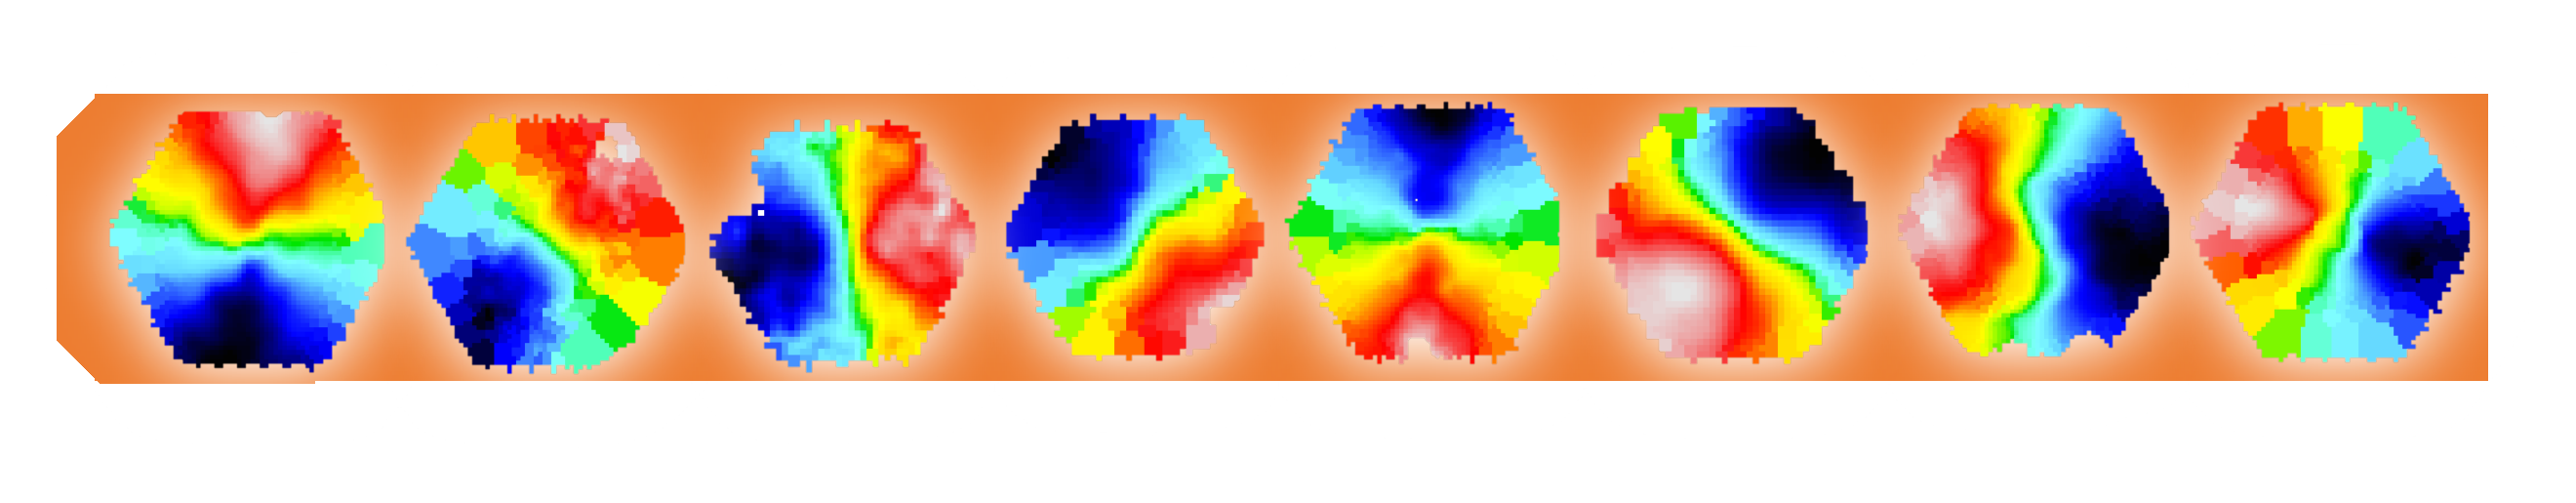
\includegraphics[height=1.39in]{thesis/latex/misalignment_MaNGA/kin_mis_chapter_heading.pdf}
\vspace{3in}

\epigraph{This chapter is predominately based on Duckworth, Tojeiro and Kraljic, in MNRAS 492, Issue 2, 2020, however also is also partially based on sections of Duckworth, Tojeiro, Kraljic, Sgr\'o, Wild, Weijmans, Lacerna and Drory, in MNRAS, 448, Issue 1, 2019. Here, we introduce kinematic misalignment and investigate the relationship of kinematically misaligned galaxies with morphology, angular momentum and gas content in both observations and simulations.} 

\section{Introduction}
%Studies in more recent IFS surveys and simulations have demonstrated the close interlink between stellar angular momentum, stellar mass and morphology suggesting that late types and early type fast rotators form a continuous sequence rather than from fundamentally different formation pathways \citep[][]{cortese2016, lagos2017, graham2018}. Remarkably, despite the highly non-linear processes involved, current cosmological surveys predict that the stellar angular momentum in rotationally supported galaxies at $z=0$ is still conserved from that of the dark matter halo \citep[e.g.][]{genel2015}. 
While the stellar continuum is often considered for studies of angular momentum, optical IFS observations also provide kinematic information of the ionized gas in the galaxy. In the basic picture of TTT, stars form from the collapsing gas leading to the expectation that they inherit its dynamics and hence galaxies have coherent rotation between their stars and gas. Unsurprisingly galaxy evolution is complex and galaxies seldom form in isolation, resulting in a significant proportion of galaxies with decoupled rotation between their stars and ionized gas. 

An offset between the rotation of stars and ionized gas has been motivated to be of external origin \citep[see][]{sarzi2006,davis2011a}. The ability of a given galaxy to accrete cold gas determines its continued ability to form stars and hence dictate where it falls amongst the Hubble sequence. Accreted gas, however, has many origins (such as filamentary `cold mode' accretion from the cosmic web, mergers or additionally cooling flows from a shocked hot halo) however is converted into stars within typical depletion timescales of order gigayears \citep{davis2016}. 
For material stripped in mergers or for shocked gas accreting through cooling flows, a natural consideration is that the accretion may not be necessarily aligned with the angular momentum of the benefiting galaxy \citep[e.g.][]{davis2011, lagos2015}. Misalignment can be considered to be a transient property as torques from the stellar component continually act to realign the gas component which can only be opposed by sustained misaligned accretion \citep[][]{vdvoort2015, davis2016}. 

Understanding the origin and nature of galaxies with decoupled star-gas rotation (kinematic misalignment - used interchangeably) has been the focus for several recent works. \citet{davis2011a} found that $\sim 36$\% of ETGs exhibit misalignment between their star and gas rotation (i.e. difference of at least 30$^{\circ}$ between rotational axes) within the volume-limited sample of ATLAS\textsuperscript{3D} \citep{atlas3d}. This fraction increases when considering field ETGs, giving a first suggestion at an environmental dependence. For late types, \citet{chen2016} first investigated star forming galaxies with counter-rotating stars and gas (i.e. difference of at least 150$^{\circ}$ between rotational axes), a far rarer occurrence ($\sim$2\%), finding a clear boost in star formation in central regions. This suggests that the processes leading to significant misalignment are also inherent in cancelling angular momentum, enabling increased gas in-flows to nuclear regions. \citet{jin2016} extended this discussion to find that for a sample of 66 misaligned galaxies, the misalignment fraction ($> 30^{\circ}$) is dependent on properties such as specific star formation rate, stellar mass and local environment, again determining that misaligned galaxies are more isolated. 

Despite this, kinematic misalignment appears to be correlated with mergers and interactions. In CALIFA, \citet[][]{barrera2015} investigated a range of interacting galaxies (i.e. at different stages of a merger) in comparison to a non-interacting control. They demonstrate that interacting galaxies of all stages demonstrate both more significant misalignment between stars and gas represented in global position angles, but also that position angles are more likely to deviate as a function of radius for any given component. This is corroborated by \citet{li_decoupling2019} who investigated the relationship between kinematic misalignment in MaNGA and deeper photometry in the Dark Energy Spectroscopic Instrument (DESI) Legacy Imaging Surveys \citep{dey2019}. They find that up-to 40\% of misaligned galaxies in MaNGA can be attributed to ongoing or recent mergers/interactions, underlining the importance of external processes. 

This likely represents a lower limit on the importance of interactions due to the typical timescales of misalignment. \citet{davis2016} utilise a toy model to propose that misaligned gas could relax gradually over time-scales of 1-5 Gyr. A faster time-scale of relaxation would require merger rates of $\approx 5$ Gyr\textsuperscript{-1} and hence is disfavoured. The interplay between the strength and persistence of the gas in-flow and the re-aligning torque of the stellar component dictates the exact time-scale of misalignment for an individual galaxy. The strength of a galaxy's stellar torque scales as a function of radius, with the central component of a galaxy re-aligning on a quicker time-scale than the outer regions. The persistence of misalignment has also been considered in numerical simulations. \citet{vdvoort2015} consider the evolution of a misaligned gas disc formed from a merger which removes most of the original disc. During re-accretion of the cold gas, the misaligned disc persists for approximately 2 Gyr before the gas-star rotation angle falls below 20$^{\circ}$. The sustainment of this misalignment is due to continued gas accretion for approximately 1.5 Gyr before its rate falls and the gas can realign with the stellar component on approximately six dynamical time-scales. 

In the field of kinematic misalignment, direct comparison between observations and simulations have been made in parallel during the time of this thesis work. In the SAMI survey, \citet{bryant2019} utilised misalignments for $\sim$1200 galaxies, demonstrating that morphology holds the strongest correlation with the likelihood of star-gas decoupling, ahead of local environment and stellar mass. 

A direct comparison of this observational SAMI sample to the cosmological simulation of \texttt{Horizon-AGN} is made by \citet{khim2019}. They find that a selected subsample of galaxies in \texttt{Horizon-AGN} reproduces the general trends of misalignment fraction with morphology and stellar mass. Despite this, they find that simulated galaxies in clusters are far more likely to be misaligned than their observed counterparts. Finally, there is observational evidence \citep[e.g.][]{davis2016, chen2016} that counter-rotation between stars and gas (usually defined as $> 150^{\circ}$ is a stable-state leading to a boost in galaxies with these typical offsets. This isn't reproduced by \texttt{Horizon-AGN}, likely due to the spatial resolution of the simulation (roughly 1kpc) which is difficult to resolve thin disks and hence realistically balance the effect of stellar torques and relaxation. A caveat in the work of \citet{khim2019} is that they do not aim to directly recreate the SAMI sample or mock observations, which convolutes physical differences between observation and simulation with discrepancies due to measurement and how properties are computed. 

Finally, \citet{starkenburg+19} considered the nature of counter-rotation ($\mathrm{> 90^{\circ}}$ between rotational axes of stars and gas) in low mass galaxies in Illustris. They identify the key role of gas loss through black hole (BH) feedback and flyby interactions to enable misalignment through re-accretion of misaligned material. The mechanisms for decoupling gas are not fully determined and are likely a combination of both external and internal processes, both of which are seen to also shape the stellar angular momentum content of galaxies at $z=0$. To understand how these non-linear processes relate both to angular momentum retention from the dark matter halo and how this propagates to star-gas decoupling, a combination of both observations and simulations are required. 

In this Chapter, we investigate kinematic misalignment in the MaNGA IFS survey (\S\ref{sec:manga_kin_mis}), and make direct comparison to the hydrodynamical simulation of IllustrisTNG (\S\ref{sec:tng_kin_mis}). Specific to observations; in \S\ref{sec:manga_intro} we introduce the MaNGA survey and associated data output, before describing the methodology in defining kinematic misalignment. \S\ref{sec:data_obs} gives a description of the additional data catalogues used in this work and \S\ref{sec:results_obs} describes the observational properties of misaligned galaxies, before summarising our observational findings in \S\ref{sec:summary_manga}. In the second half of the chapter, we describe the construction of a mock MaNGA sample created in IllustrisTNG and make direct comparisons to the observational results, before investigating the evolution histories of angular momentum. Specific to simulations; \S\ref{sec:sim_data_TNG} introduces the IllustrisTNG simulation and the creation of the mock observational sample. \S\ref{sec:manga_tng_comp} makes direct comparison between IllustrisTNG and MaNGA. \S\ref{sec:tng_ang_mom_evo} describes the evolutionary histories of angular momentum for the misaligned galaxies before summarising in \S\ref{sec:tng_summary}. We discuss the implications of the chapter in \S\ref{sec:tng_discussion}.

\section{In MaNGA} \label{sec:manga_kin_mis}
\subsection{The MaNGA survey} \label{sec:manga_intro}
Set to complete in 2020, the MaNGA survey is designed to investigate the internal structure of $\sim$10000 galaxies in the nearby Universe. By design, the complete sample is unbiased towards morphology, inclination and colour and provides a near flat distribution in stellar mass. 
MaNGA is one of three programs in the fourth generation of the Sloan Digital Sky Survey (SDSS-IV) which enables detailed kinematics through integral field unit (IFU) spectroscopy. MaNGA uses the SDSS 2.5 metre telescope in spectroscopic mode \citep{gunn2006} with the two dual-channel BOSS spectrographs \citep{smee2013} and the MaNGA IFUs \citep{drory2015}. MaNGA provides spatial resolution on kpc scales (2'' diameter fibres) while covering 3600-10300$\mathrm{\mathring{A}}$ in wavelength with a resolving power that varies from R$\sim$1400 at 4000$\mathrm{\mathring{A}}$ to R$\sim$2600 at 9000$\mathrm{\mathring{A}}$. 

MaNGA observations use SDSS style plates, where bundles of optical fibres are plugged into the plate corresponding to the position of the target galaxy in the observational field. A dithered pattern is employed for each target field (plate), which simultaneously observes galaxies through 17 fibre-bundles of 5 distinct sizes. Any incomplete data release of MaNGA should therefore be unbiased with respect to IFU sizes and hence a reasonable representation of the final sample scheduled to be complete in 2020.

The majority of observations contribute to one of the three main subsets: the Primary sample, the Secondary sample and the Colour-Enhanced supplement. All sub-samples observe galaxies to a minimum of $\sim 1.5$ effective radii ($\mathrm{R_{e}}$) with the Secondary sample increasing this minimum to $\sim 2.5 \mathrm{R_{e}}$. The Colour-Enhanced supplement fills in gaps of the colour-magnitude diagram leading to an approximately flat distribution of stellar mass. A full description of the MaNGA observing strategy is given in \citet{law2015obs,yan2016obs}. The raw observations are processed by the MaNGA Data Reduction Pipeline (DRP) as described in \citet{law2016drp, yan2016spec}. The fibre flux and inverse variance is extracted from each exposure, which are then wavelength calibrated, flat-fielded and sky subtracted.

MaNGA releases data periodically in the form of MaNGA Product Launches (MPL), both increasing the number of observed galaxies and updating the data processing. In the following chapters we use data from MPL-6 and MPL-8 referring to the sixth and eighth Product Launches.
% Include a figure showing the distribution of NSA, MaNGA targets, MPL-6 and MPL-8.
% Also include figure of bundle sizes?
 
\subsubsection{Velocity fields} \label{sec:vel_fields_intro}
The MaNGA Data Analysis Pipeline \citep[DAP][]{westfall2019,belfiore2019} provides science-ready processed data for MaNGA observations. Some example outputs include; spaxel-by-spaxel coordinate information based on the isophotal ellipticities from the NASA-Sloan Atlas, S/N measurements, binned spectra, stellar kinematics and stellar-continuum models, emission-line properties and models, and spectral-index measurements. Kinematics are easily accessible as 2D maps which we use for stellar and gas velocity fields in the following analysis. A complete discussion can be found in \citet{westfall2019,belfiore2019}, however we will summarise the key points concerning stellar and gas velocity fields here.

The DAP extracts stellar kinematics using the Penalised Pixel-Fitting (pPXF) method \citep{cappellari2004,cappellari2017}. The DAP fits the stellar continuum of each spaxel to extract the line of sight velocity dispersion and then fits the absorption-line spectra from a set of 49 clusters of stellar spectra from the MILES stellar library \citep{sanchez2006,falcon2011}. Before extraction of the mean stellar velocity, the spectra are spatially Voronoi binned to $g$-band \textit{S/N} $\sim$ 10, excluding any individual spectrum with a $g$-band \textit{S/N} < 1 \citep{cappellari2003}. This approach is geared towards stellar kinematics as the spatial binning is applied to the continuum \textit{S/N}, however, we note that unbinned and Voronoi binned velocity maps produce similar results. 

Ionized gas kinematics are extracted by the DAP through fitting a Gaussian to the H$\alpha$-6564 emission line, relative to the input redshift for the galaxy. This velocity is representative for all ionized gas, since the parameters for each Gaussian fit to each emission line are tied during the fitting process. These velocities are also binned spatially by the Voronoi bins of the stellar continuum. 

\subsubsection{Kinematic misalignment} \label{sec:kin_mis}
We estimate the two dimensional global position angle (PA) of the stellar and H$\alpha$ gas velocity fields using the \texttt{FIT\_KINEMATIC\_PA} routine outlined in Appendix C of \citet{krajnovic2006}. By default this finds the angle corresponding to the bisecting line which has greatest velocity change along it (i.e. the angle of peak rotational velocity). We choose this angle to be found from sampling at 180 equally spaced steps. This is measured counter-clockwise from the north axis, however, it does not discriminate between the blueshifted and redshifted side since it is only defined up to 180$^{\circ}$. As a result, velocity fields with a difference of 180$^{\circ}$ PA would appear to be aligned. To solve this we identify the direction of rotation and re-assign a consistent PA: defined as the axis of rotation approximately 90$^{\circ}$ clockwise from the blueshifted side. This angle now spans 360$^{\circ}$ allowing an automatic detection of misaligned gas and stellar components. The offset angle between kinematic components is defined as: 
\begin{equation} \label{eq:delPA}
\mathrm{\Delta PA = |PA_{stellar} - PA_{H\alpha}|. }
\end{equation}
We define galaxies with $\Delta$PA > 30$^{\circ}$ to be significantly kinematically misaligned. An example of an aligned and a misaligned galaxy is shown in Figure \ref{fig:cutout_wIFU}. 

\begin{figure*}
    \centering
	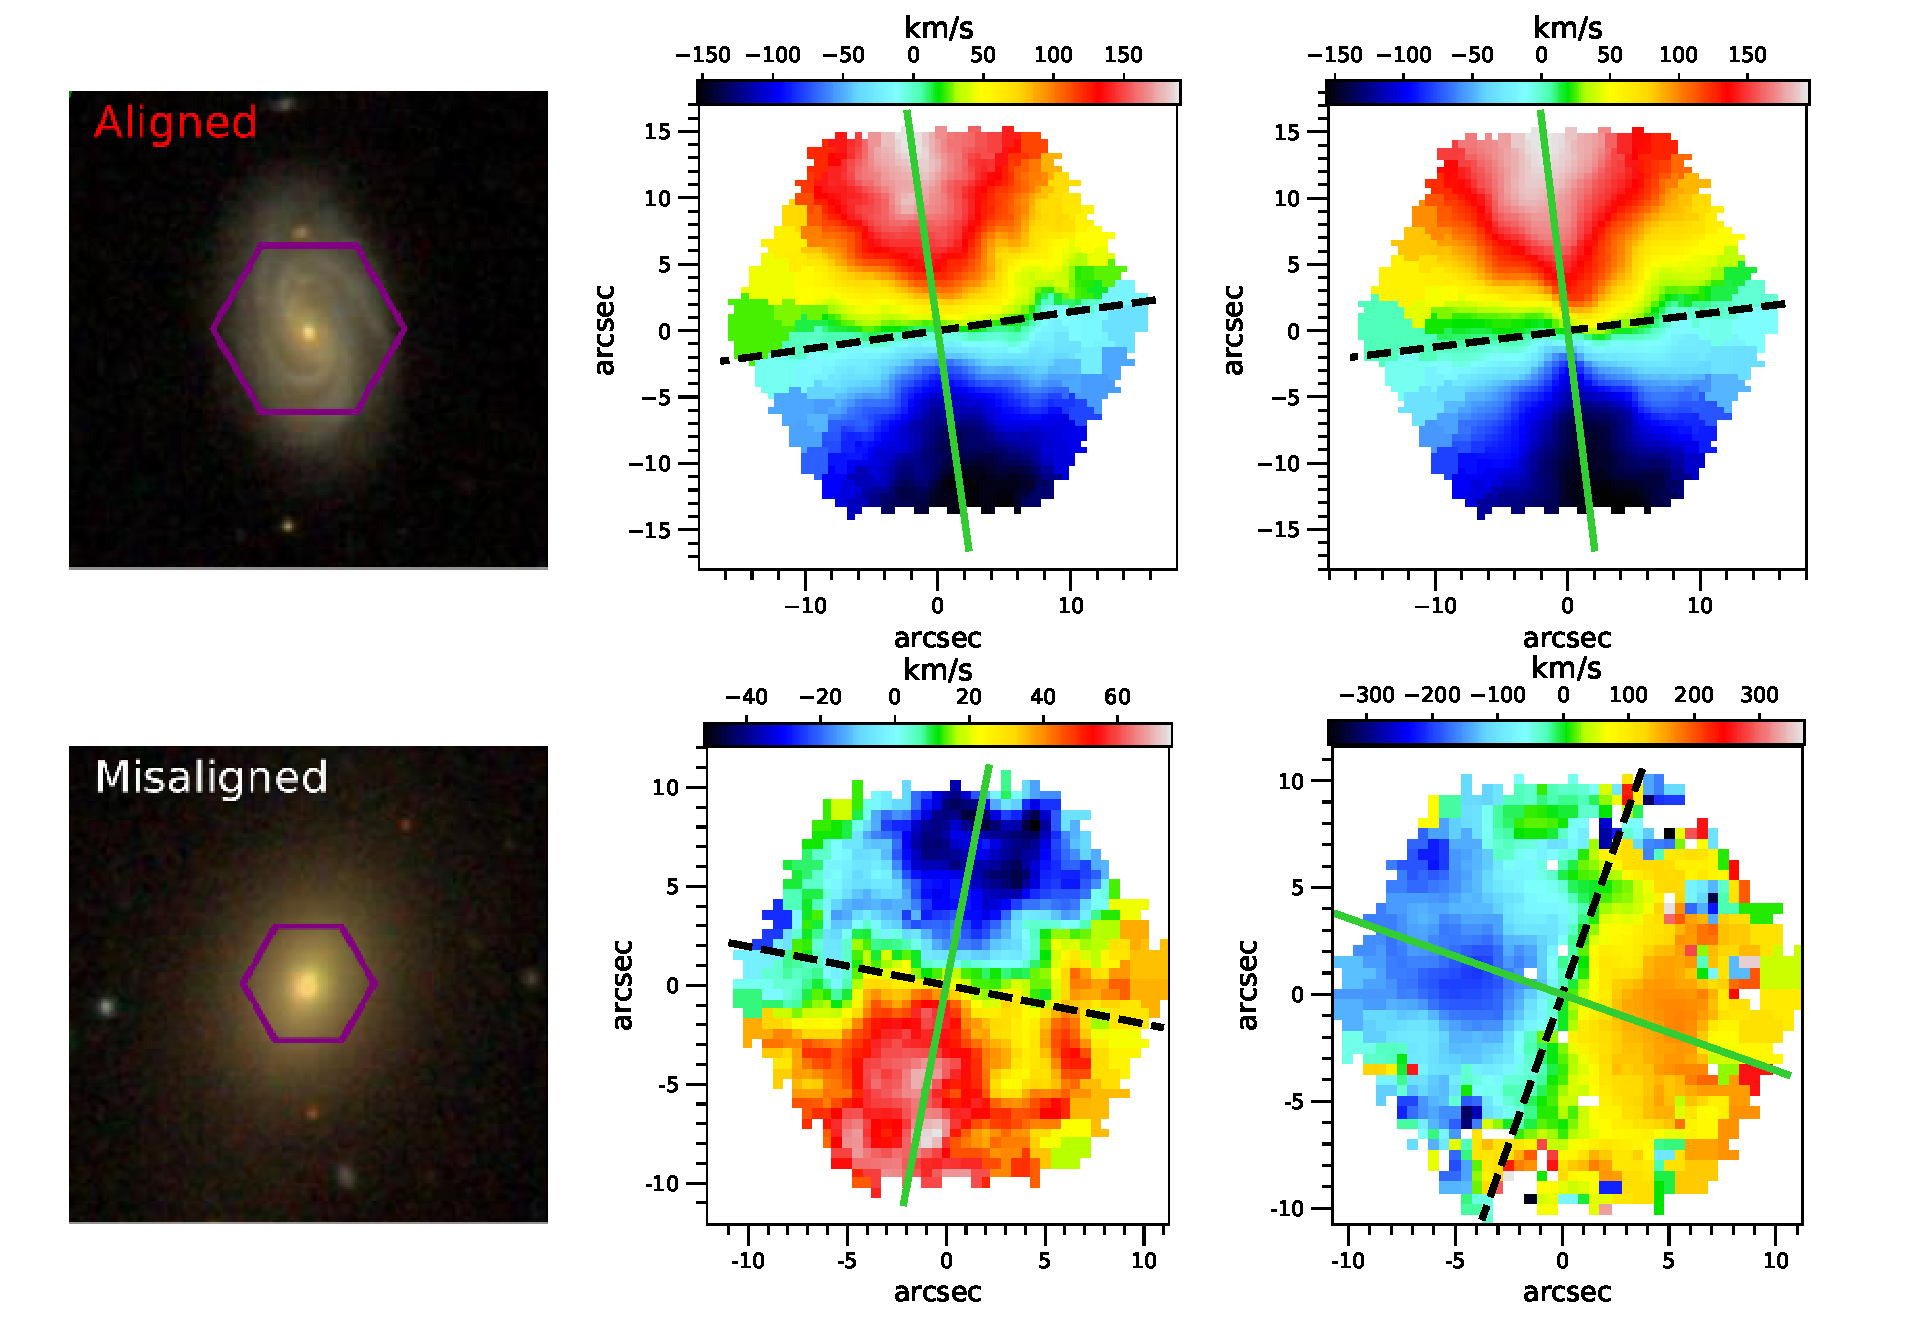
\includegraphics[width=0.8\linewidth]{thesis/latex/misalignment_MaNGA/cutout_wIFU_revised.pdf}
    \caption[Examples of a kinematically aligned (top) and misaligned (bottom) galaxy defined by $\Delta$PA.]{Examples of a kinematically aligned (top) and misaligned (bottom) galaxy defined by $\Delta$PA. From left to right, the panels show (i) the original SDSS cutout of surrounding field with the MaNGA IFU footprint overlaid in purple, (ii) stellar velocity field and (iii) $H\alpha$ (gas) velocity field. The velocity fields are marked by a defined PA (green solid line) and axis of rotation (black dashed line). The galaxy in the bottom row is misaligned due to it having $\Delta$PA > 30$^{\circ}$. The colour-bars represent the velocity fields in km/s and the galaxies are orientated so that up corresponds to North and right to East.}
    \label{fig:cutout_wIFU}
\end{figure*}

To improve the reliability of the PA fit, we apply a few additional filters to the velocity fields. While foreground stars are flagged within observations, background/small neighbouring galaxies can remain within the IFU footprint. This is a problem for fitting a global position angle since it naturally interprets other material as part of the target galaxy's observation and interpolates between the regions. We remove all disconnected regions smaller than $10\%$ of the target galaxy's footprint. In addition we sigma clip the velocity field and remove all spectral pixels (spaxels) above a $3\sigma$ threshold.

Our choice to take $\Delta$PA > 30$^{\circ}$ as significantly kinematically misaligned is a conservative selection to ensure we are selecting galaxies undergoing external interaction. There is evidence to suggest that accretion drives misalignment past $\Delta$PA = 30$^{\circ}$. \citet{lagos2015} found that using solely galaxy mergers as the source for misaligned cold gas only predicts 2\% of ETGs to have $\Delta$PA > 30$^{\circ}$ using GALFORM, in comparison with the misaligned field ETG fraction found in ATLAS\textsuperscript{3D} of 42 $\pm$ 6\%  \citep{davis2011a}. This puts a lower level of importance on gas accretion. Our choice can be justified as follows. Firstly, we are using ionized gas as a proxy for the distribution and accretion of cold gas. \citet{davis2011a} find that the typical difference between the PAs of cold gas (CO) and ionized gas can be described by a Gaussian distribution centred on 0 with a standard deviation of 15$^{\circ}$ for 38 CO bright galaxies in ATLAS\textsuperscript{3D}. While indicating ionized gas is a reasonable estimator for cold gas, splitting $\Delta$PA = 30$^{\circ}$ accounts for the scatter in this relationship. Secondly, this should avoid spurious misalignments arising from errors in the fit of $\Delta$PA. While our model errors are low, they are likely an underestimation since they do not include more complex motions. However, selecting a lower split in $\Delta$PA would only be affected by the increased likelihood of internal processes being dominant, rather than the inaccuracy of fitting. Any threshold in $\Delta$PA becomes a trade off between sample size and contamination probability. Altering our cut in $\Delta$PA to be 20$^{\circ}$, 40$^{\circ}$ or similar does not change any of the conclusions drawn in this chapter.

\subsubsection{Error estimation}
It is an important point to constrain the errors of our PA fits, so we can reliably trust cuts in $\Delta$PA to select galaxies which are significantly kinematically misaligned and hence have had external interaction. Here, we construct two component model velocity maps for each stellar and gas component of every MPL-6 observation in order to estimate typical errors on $\Delta$PA from \texttt{FIT\_KINEMATIC\_PA} for the MaNGA sample. \red{MPL-6 corresponds to a total of 4633 unique galaxy observations.}

Errors using the \texttt{FIT\_KINEMATIC\_PA} routine have been previously estimated for molecular gas velocity fields in ATLAS\textsuperscript{3D} \citep{davis2011a}. Model velocity fields with a known PA were constructed using an empirical galaxy rotation curve and combined with Gaussian noise matched to the signal-to-noise ratio of the data. A typical scatter of $\approx10^{\circ}$ was found due to varying inclination and angular resolution for the velocity fields.

\subsubsection{Circular velocity}
To find the typical error on $\Delta$PA for galaxies in MaNGA, we create model velocity maps for both the stellar and gas components of each MPL-6 observation. In each instance the basic construction of the model follows Section 4 of \citet{krajnovic2006}. Each velocity field comprises of a two-component Hernquist potential which provides a basic circular velocity given by,
\begin{equation}
\mathrm{V_c = \frac{\sqrt{GMr}}{r+r_0}}
\end{equation}
where $G$ is the gravitational constant, $M$ is the total mass and $r_0$ is the core radius of each component respectively \citep{hernquist1990}. We use a two-component model to include the relative strengths of both disc and bulge each with distinct effective radii, $R_e$. We fix $r_0$ to be 5 and 15 (units: $arcsec$) and $\sqrt{GM}$ to be 850 and 1500 (units: $km s^{-1} arcsec^{1/2}) $ for the bulge and disc components respectively. These individual components are light weighted by model sersic flux profiles according to,
\begin{equation}
\mathrm{I(r) = I_0 e^{-\left(\frac{R}{R_e}\right)^{n_s}}}
\end{equation}
where $I_{0}$ is the peak flux and $n_s$ is the sersic index which is set to 1 and 4 for the disc and spheroidal components respectively. Since we do not have bulge-disc decompositions, we lack individual effective radii for both the bulge and disc components. Instead, we set the bulge and disc effective radii to be 0.5$R_e$ and 1.5$R_e$, where $R_e$ is the effective radius estimated by an elliptical petrosian fit taken from the NSA targeting catalogue. 

\subsubsection{Calibration}
For each MaNGA galaxy a basic velocity field model is constructed using this template. The axes of the model velocity field are then scaled according to the inclination, $i$, which is estimated from the $b/a$ ratio taken from the NSA catalogue and is also used to scale the fraction of rotational velocity along the line-of-sight. The velocity field for each component, ($j=bulge,disc$), in polar coordinates $(r,\phi)$ is then described by,
\begin{equation}
\mathrm{V(r,\phi) = \frac{I_{j}(r)}{I_{tot}(r)}V_{c}(r)\cos(\phi+\theta_{j})\sin(i)}
\end{equation}
where $\theta_j$ is the input kinematic position angle. We set $\theta_{bulge} = \theta_{disc}$ for simplicity, however, we do note that galaxies with more complex orbital motions may increase the typical error. The position angle for both bulge and disc is simply taken to be the opening angle of the galaxy (direction of major axis taken from NSA catalogue). 

In order to imitate a MaNGA observation, the model velocity field is sampled at the spatial resolution of the corresponding IFU bundle and projected into the original shape of the actual observation for H$\alpha$ and stellar maps respectively. Gaussian noise is drawn for each spaxel from a normal distribution with the standard deviation taken from the errors on the actual observation. In addition, these model velocity fields are then Voronoi binned to match the original observation.

Example stellar and H$\alpha$ velocity fields generated from these models are shown in Figure \ref{fig:sim_ifu} with comparison to the actual observation. As expected, the model velocity fields frequently recreate observations well but struggle to encompass more complex motion. For this reason, our models should make a reasonable prediction on the typical $\Delta$PA errors intrinsic to MaNGA observations.

\begin{figure}
    \centering
	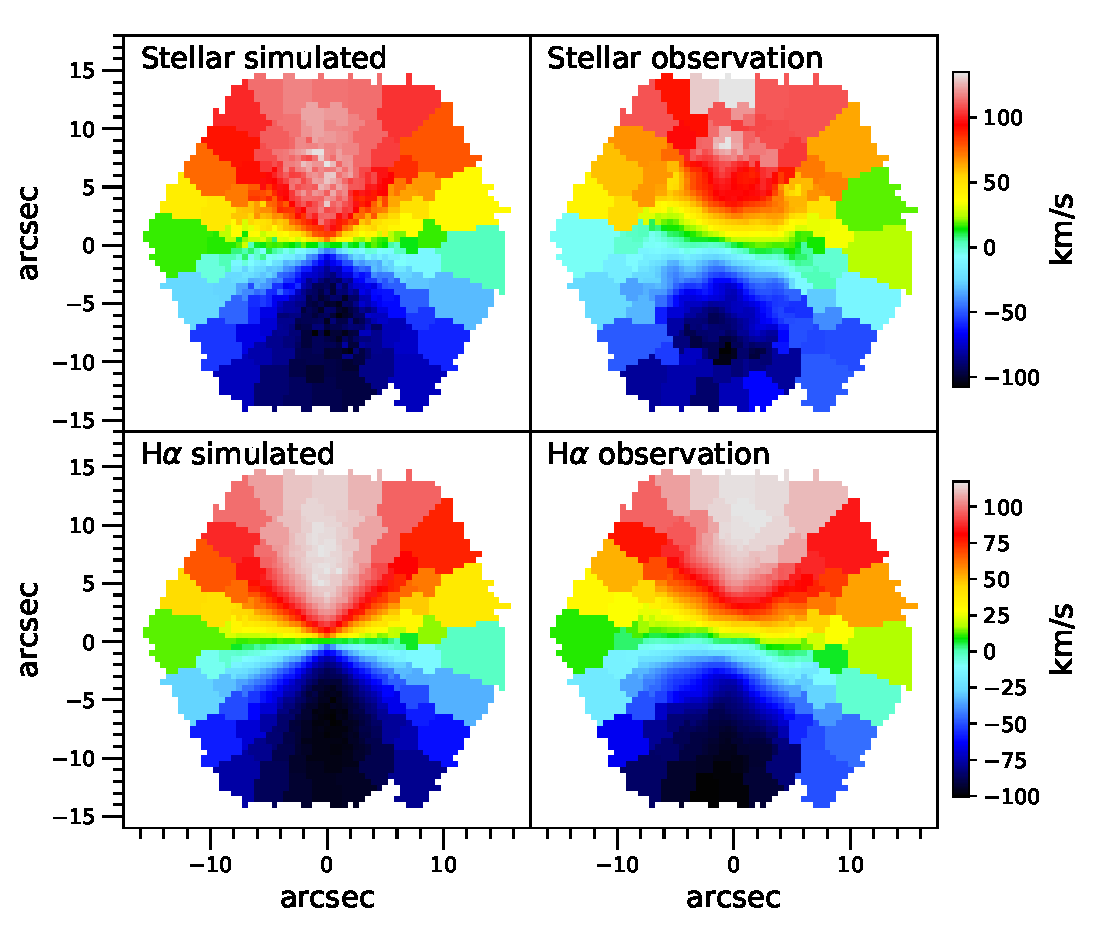
\includegraphics[width=0.7\linewidth]{thesis/latex/misalignment_MaNGA/obs_sim_IFU.pdf}
    \caption[Comparison velocity maps for simulation (left column) and observation (right column).]{Comparison velocity maps for simulation (left column) and observation (right column). Stellar (H$\alpha$) component velocity maps are shown on the top (bottom) row with the associated velocity colourbars.}
    \label{fig:sim_ifu}
\end{figure}

\subsubsection{Typical errors}
We construct model velocity fields for all non-critically flagged MPL-6 galaxies, inclusive of the $\Delta$PA sample used in this work. Figure \ref{fig:model_errors} shows the cumulative probability distribution for the range of $0-5^{\circ}$ where the majority of errors fall. We find that \texttt{FIT\_KINEMATIC\_PA} gives a typical combined (stellar and gas) mean error of $1.3^{\circ}$. While this is an underestimation of true $\Delta$PA errors for a sample of galaxies including those with more complex velocity fields, it is indicative that selecting a cut at $\Delta$PA = 30$^{\circ}$ should be robust to identifying galaxies with external interaction. \todo{Has python version of fit kinematic pa been updated to include this?}

\begin{figure}
    \centering
	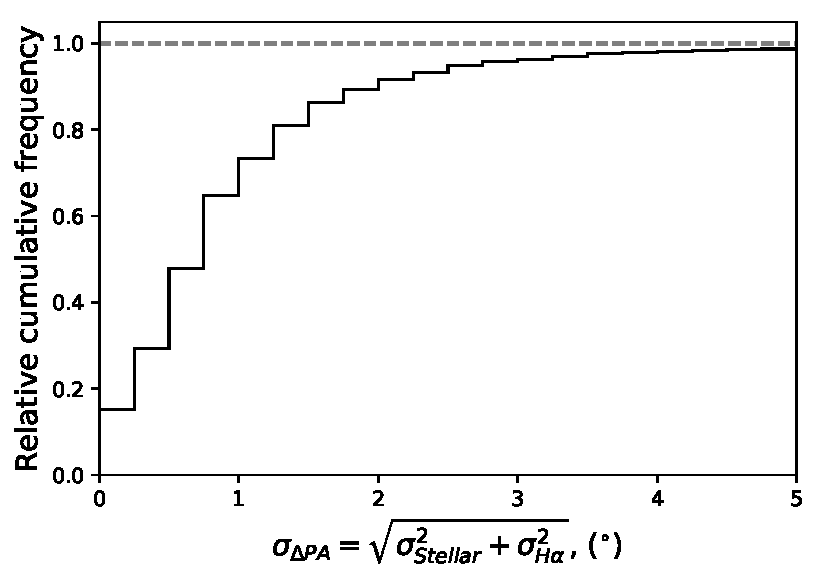
\includegraphics[width=0.6\linewidth]{thesis/latex/misalignment_MaNGA/cumulative_model_errors.pdf}
    \caption{Cumulative histogram of errors for fitting kinematic PA to model maps for the all non-critically flagged MPL-6 galaxy observations.}
    \label{fig:model_errors}
\end{figure}

\subsubsection{Visual Classification}
Global position angles are only well defined for coherently rotating velocity fields. Those with a decoupling between inner and outer regions due to warps or kinematically decoupled cores (KDCs) are poorly described by global PAs. To select a clean sample of galaxies with well defined global PAs, we visually classify all of the velocity fields after pre-processing and PA fitting. Both stellar and H$\alpha$ velocity fields are characterised into 3 categories;
\begin{itemize}
    \item Dominant coherent rotation and well defined PA.
    \item Dominant coherent rotation but with more noise or more complex motion resulting in a usable PA fit but with higher typical errors. Highly inclined velocity fields with a higher likelihood of inaccurate PAs fits are included in this category. 
    \item Do not use.
\end{itemize}

Kinematic features are also identified. Both stellar and H$\alpha$ velocity fields are classified into;
\begin{itemize}
    \item Kinematically decoupled core (i.e. those with a central component that rotates in a different direction ($> 30^{\circ}$) with respect to the overall galaxy rotation).
    \item Warp (velocity field of central region is warped with respect to outskirts. This may be due to a bar, oval shaped structures in the disc (oval distortions) or accretion of fresh material with different angular momentum to the bulk rotation).
    \item Merger (ongoing merger or neighbour identified within IFU. Only those with obvious disruption are followed up in photometry).
    \item No features.
\end{itemize}
The majority of those with kinematic features have poorly defined global PAs and hence are flagged as do not use for the previous flag. The galaxies we refer to as `warped' represents a combination of galaxies with bars, oval distortions and differential rotation in the disc \citep[e.g.][]{barrera2014}. We direct the reader to \citet{stark2018} for an approach to separate the galaxies we refer to as warps. In this work, we enforce axisymmetry for our sample and hence make no use of galaxies that have significant variations in their PA as a function of radius.

For studies of quenching it may be useful to consider galaxies that have defined stellar rotation but lack coherent motion in the ionized gas. For galaxies that have usable PAs for the stellar velocity but unusable PAs for the ionized gas, we define a further classification of the gas velocity field;
\begin{itemize}
    \item Depletion (seen as empty spaxels signifying lack of gas, usually in central regions)
    \item No clear rotation (map has no clear rotation or is noise dominated)
    \item Partial rotation (partial coherent rotation in the velocity field, however there are significant regions with incoherent motion or noise domination)
    \item No clear characteristics/ No gas.
\end{itemize}
We note there is a clear overlap between the classifications for depletion and no clear rotation, since velocity fields are often a combination of these two features. 
%The total numbers for each classification in each category are summarised in Table \ref{tab:kin_class}. 
Examples of PA fits (see \S\ref{sec:def_kin_mis} for calculation) with the associated photometry for various kinematic classifications is given in Figure \ref{fig:mis_grid}. Examples of galaxies that are kinematically aligned, misaligned, have a stellar kinematically decoupled core, have a warped H$\alpha$ velocity field and have clear stellar rotation but depleted ionized gas/ no rotation are shown respectively.

\begin{figure*}
    \centering
	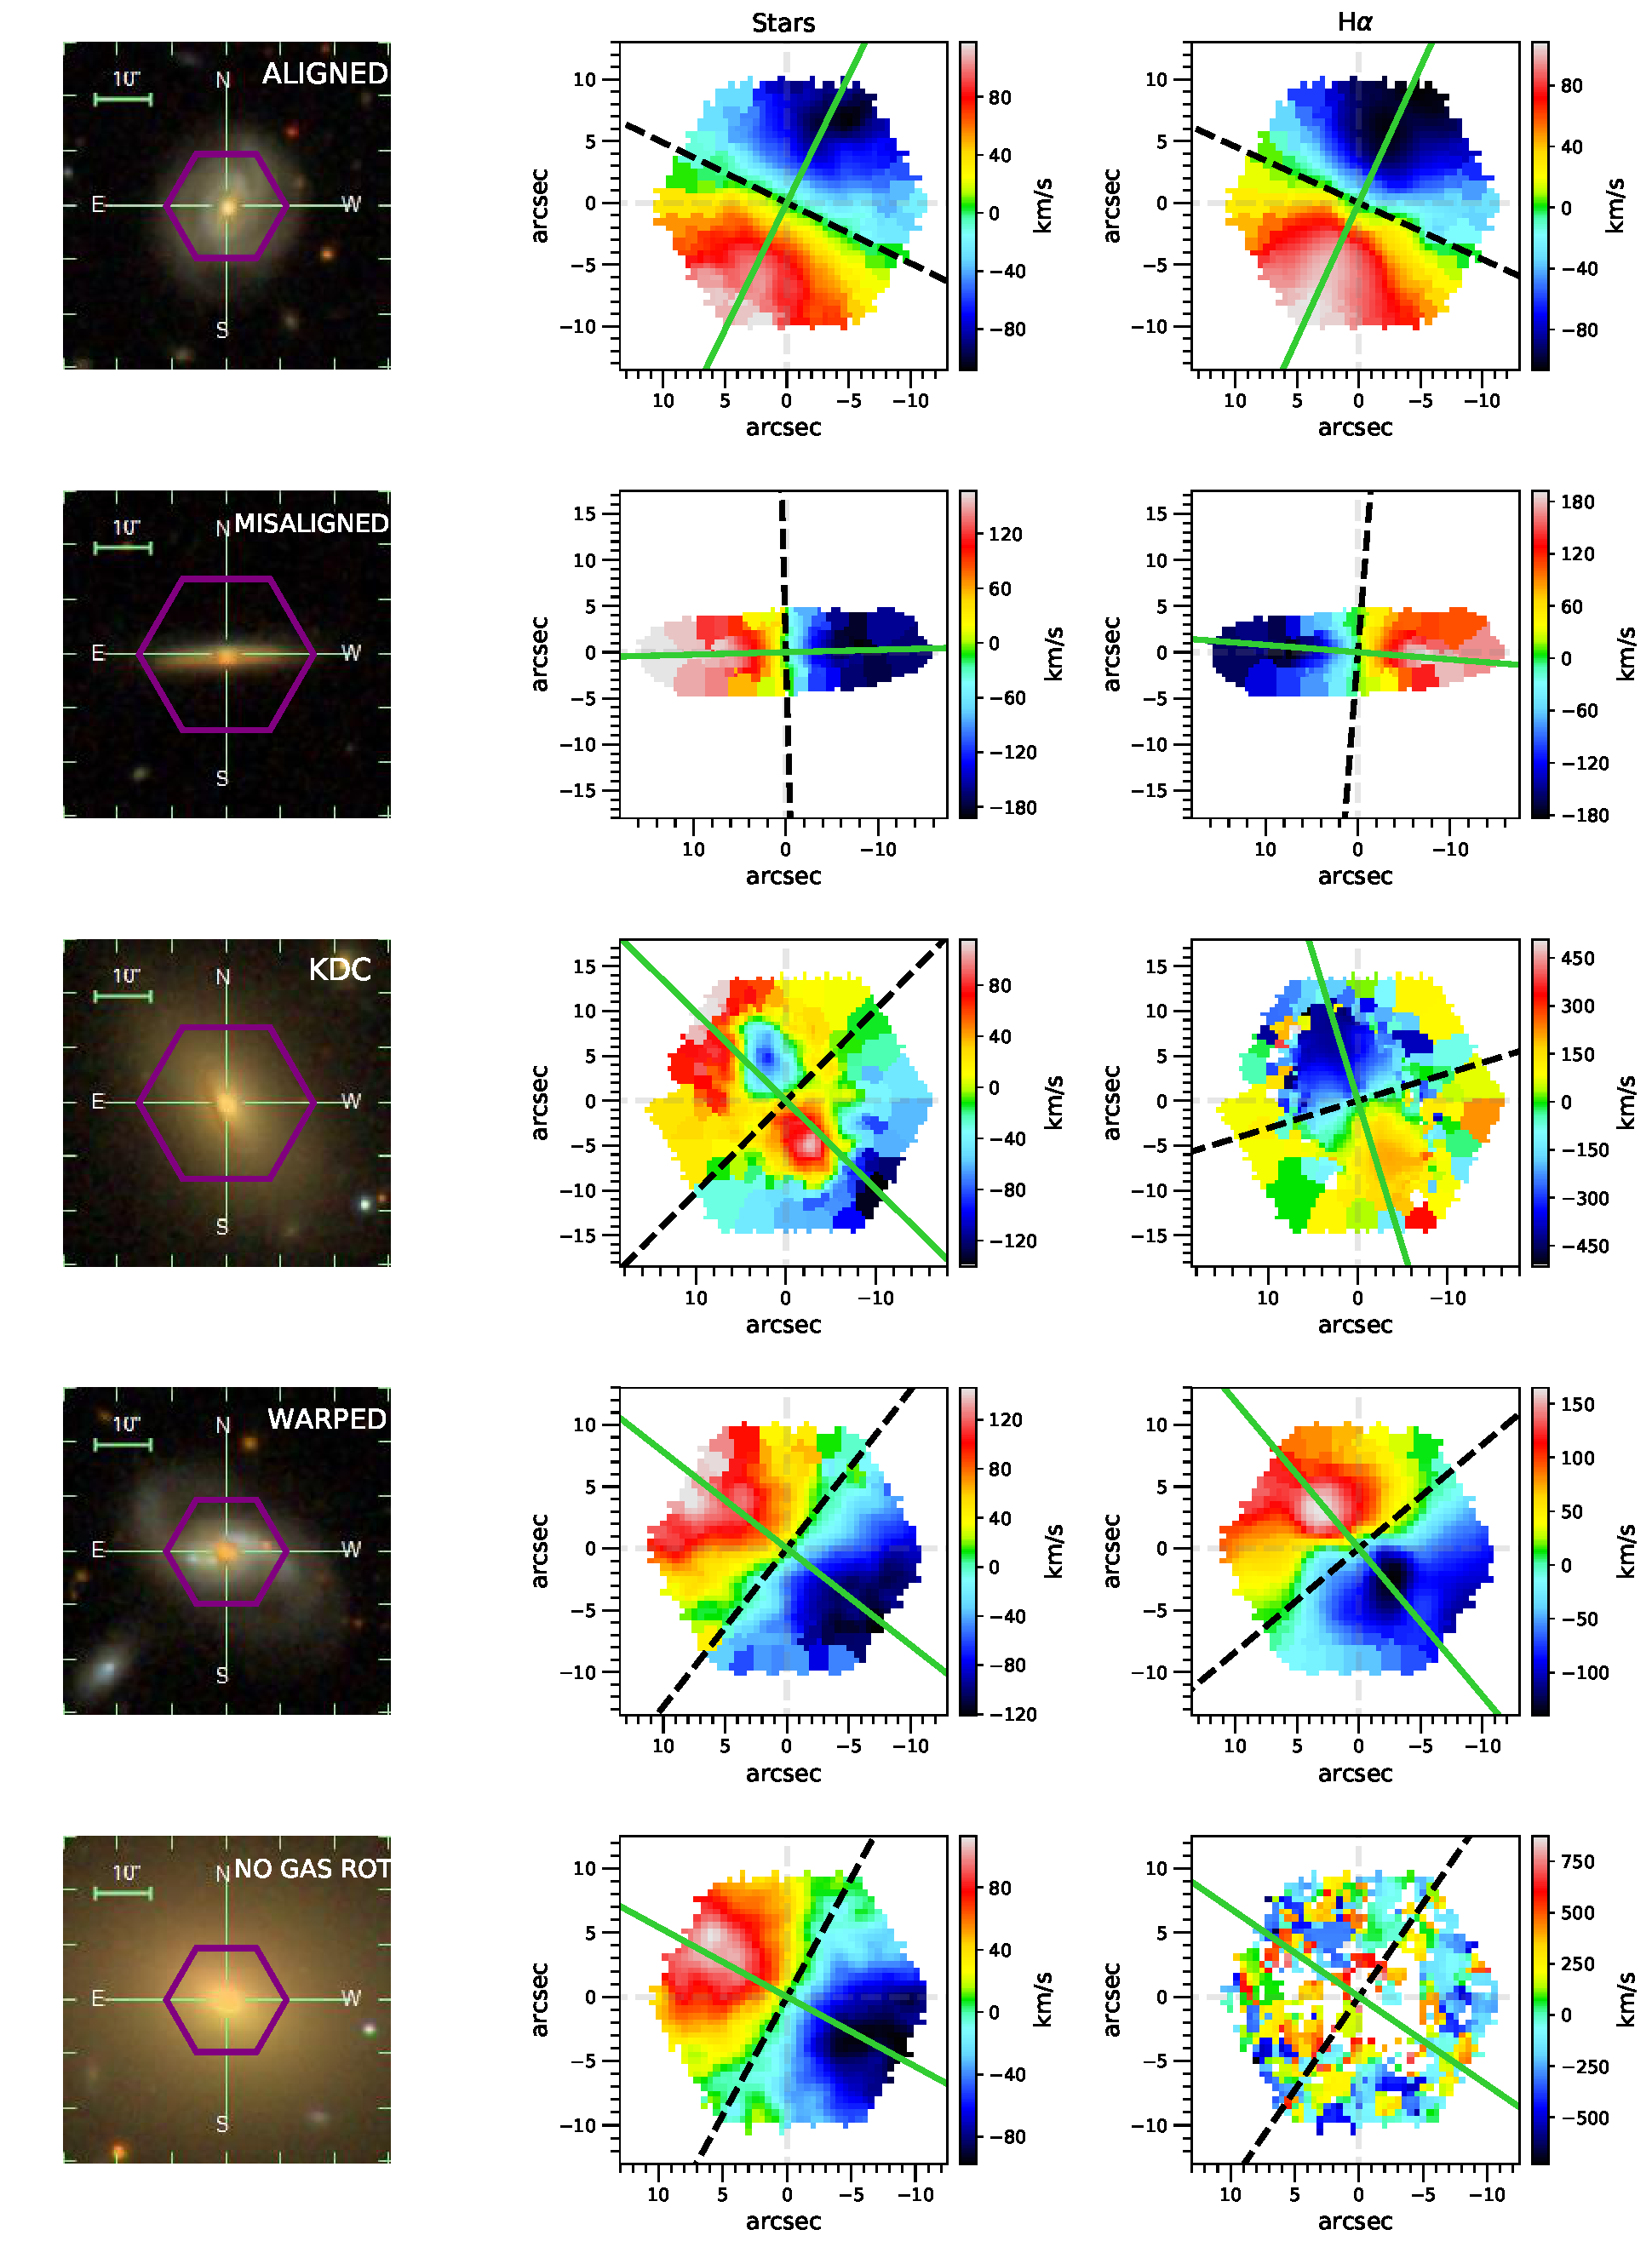
\includegraphics[width=0.93\linewidth]{thesis/latex/misalignment_MaNGA/misalignment_grid.pdf}
    \caption{Examples of PA fits for galaxies with different kinematic classifications. For each galaxy (row), we show the photometry taken from SDSS with the MaNGA IFU observation footprint overlaid in purple (left), the stellar velocity field (middle) and the H$\alpha$ velocity field (right). The kinematic PA fits (see \S\ref{sec:def_kin_mis}) are shown on the velocity fields (green solid line) with the axis of rotation (black dotted line). The kinematic classifications from top to bottom are; (a) PLATEIFU: 7958-6101, kinematically aligned near face on; (b) PLATEIFU: 8465-12704, counter-rotating near edge on; (c) PLATEIFU: 9868-12704, with a KDC in the stellar velocity; (d) PLATEIFU: 8252-6103, with a warped H$\alpha$ velocity field with respect to the stellar; (e) PLATEIFU: 10219-6102, with a centrally depleted/missing H$\alpha$ velocity field but coherent rotation in the stellar.}
    \label{fig:mis_grid}
\end{figure*}

\subsection{Data} \label{sec:data_obs}
This section describes the catalogues crossed matched with the MaNGA sample to seperate galaxies based on optical morphology and group membership.

\subsubsection{Morphology} \label{sec:morph_def_obs}
We classify the morphology of MaNGA galaxies through the formalism laid out by the citizen science project; GalaxyZoo2 \citep[GZ2;][]{willett2013}. GZ2 provides visually identified morphologies (and also measures finer morphological features e.g. bars, bulge size and edge-on discs) for 304,122 galaxies drawn from SDSS. GZ2, however, is not complete for the MaNGA sample and has been combined with an unpublished version; GalaxyZoo4 to provide a consistent set of definitions for all MaNGA targets (see \url{https://www.sdss.org/dr15/data_access/value-added-catalogs/?vac_id=manga-morphologies-from-galaxy-zoo}). 

In a nutshell, GZ2 provides morphological classification through a decision tree of questions. Further questions are dependent on the answer to the previous to characterise a certain morphological type and identify finer features (see Figure 1 in \citet{willett2013} for this flowchart). From this, a table of vote fractions for each question combined with the total number of votes dictate a reliably sampled galaxy population with a set of desired morphological features. Votes by individuals are debiased (weighted) based on their reliability in comparison to known answers to the questions.

The first question in the decision tree 'Is the galaxy smooth and rounded with no sign of a disc?', allows categorisation into broad ETGs and LTGs. We select galaxies with a debiased vote fraction > 0.7 for smooth to be ETGs and galaxies with a debiased vote fraction of > 0.7 for disc or features to be LTGs. Defining an exact population of lenticular galaxies (S0s) is tricky through public classifications. LTGs, however, can be separated based on the dominance of the bulge with respect to the disc in GZ2 through the question 'How prominent is the central bulge, compared with the rest of the galaxy?'. \citet{willett2013} demonstrate a strong correlation between bulge dominance as defined per this question and expert classifications of T-type \citep{nair2010}. Equation 19 of \citet{willett2013} provides a linear mapping from GZ2 bulge classification to expert defined morphological T-type. Care must be taken in using this linear mapping \citep[see discussion in][]{willett2013}, however, this should be a reasonable parameterisation to coarsly separate LTGs into earlier-type (S0 - Sa) and later-type spirals (Sb - Sd). We split our LTG population at T-type = 3, to give two morphological categories; S0-Sas and Sb-Sds in addition to pure ETGs.
% We split our LTG population at T-type = 3, to give three morphological categories along with pure ETGs. 

The estimates of gas mass used here for MaNGA are derived from the Pipe3D pipeline \citep{pipe3Da, pipe3Dvac}, which uses dust attenuation within the footprint of the IFU, which methodology is described in \citet{barrera2018}.

\subsubsection{Group membership} \label{sec:group_def}
\red{either put full description here or in halo assembly section.}
To investigate different pathways leading to kinematic misalignment, we must separate galaxies into centrals and satellites. We identify groups with an adaptive halo-based group finder of \citet{yang2005,yang2007} and with improved halo mass assigning techniques \citep[see;][for details and application to SDSS]{lim2017}. In a nutshell, the group finder uses either the stellar mass or luminosity of central galaxies in addition with the $\mathrm{n^{th}}$ brightest/most massive satellite as proxies for halo mass. Galaxies are assigned to groups through an iterative process, where halo properties such as halo size and velocity dispersion are updated until membership converges. 

% For groups that are outside of the redshift limit where groups are complete final halo masses are assigned through abundance matching. Those incomplete are assigned halo masses based on the ranking between halo mass and the proxy found at the final iteration of the group finder.
% The performance of the group finder has been tested on realistic mock catalogues, showing that the halo masses of individual haloes are consistent with the true mass with a typical scatter of $\sim$0.2 dex. This scatter is similar to the commonly used group finder of \citet{yang2007}, however extends uniformly to halo masses 0.7 dex lower. 

% For this work, we use the stellar mass based halo mass proxy for the SDSS main sample. 
\citet{lim2017} do not apply the group finder to the thin strips in the Southern Galatic Cap of SDSS main due to incomplete groups resulting from close proximity to borders. MaNGA galaxies in these strips are therefore unclassified by the group finder, resulting in 5088 matched galaxies with group membership classifications into central or satellite. 

\subsection{Results} \label{sec:results_obs}
\red{redefine NGRs}
We divide our MaNGA $\Delta$PA defined population at $\Delta$PA = 30$^{\circ}$ into aligned and misaligned. In the following, we also consider galaxies with defined stellar PAs but undefined H$\alpha$ due to central depletion or incoherent rotation/dispersion domination (no gas rotation; NGRs). Figure \ref{fig:delPA_stelM} shows the distribution of stellar mass for these three populations. We see no significant difference between the aligned and misaligned galaxies, however NGRs appear to be slightly more massive. \citet{graham2018} previously demonstrated the tight correlation between stellar angular momentum and stellar mass for MaNGA ($\sim$2300 galaxies). Since NGRs and misaligned galaxies are slightly higher mass, it could be expected that they are typically less rotationally supported with respect to the $\Delta$PA defined populations. 

\begin{figure}
    \centering
	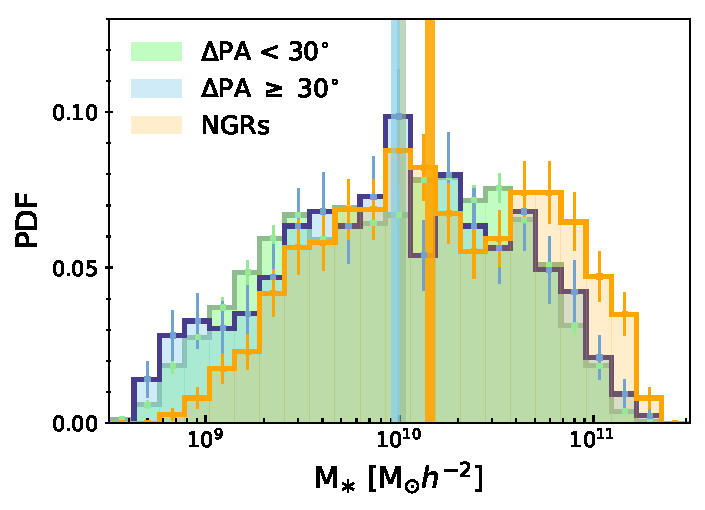
\includegraphics[width=0.7\linewidth]{thesis/latex/misalignment_MaNGA/delPA_stelM.pdf}
    \caption{Probability density distributions of stellar mass, $\mathrm{(M_{\ast}/M_{\odot})}$ for aligned galaxies ($\Delta$PA < 30$^{\circ}$) shown in green, those with high misalignment ($\Delta$PA > 30$^{\circ}$) are in blue and NGRs are in orange. Each histogram is given with Poisson errors on each bin. The vertical lines denote the corresponding distribution's median. NGRs are typically at higher stellar mass than those with aligned star and gas rotation.}
    \label{fig:delPA_stelM}
\end{figure}

Here we use the luminosity weighted stellar angular momentum estimator, $\mathrm{\lambda_R}$, taken directly from Equation 1 in \citet{emsellem2007} as
\begin{equation}
\mathrm{\lambda_{R} \equiv \frac{\langle R | V | \rangle}{ \langle R \sqrt{ V^{2} + \sigma^{2} } \rangle } = \frac{ \Sigma_{ n = 1 }^{ N } F_{ n } R_ { n } \left| V_{ n } \right| }{ \sum_{ n = 1 }^{ N } F_{n} R_{ n } \sqrt{ V_{ n }^{ 2 } + \sigma_{ n }^{ 2 } } }.}
\end{equation}
$\mathrm{\lambda_R}$ is calculated from summing over N pixels in the IFU observation within the radius of interest, $\mathrm{R}$. $\mathrm{F_{n}}$, $\mathrm{V_{n}}$ and $\mathrm{\sigma_{n}}$ are the flux, line of sight velocity and line of sight velocity dispersion of the $\mathrm{n^{th}}$ pixel. Here we present all measures of $\mathrm{\lambda_R}$ encompassing a radius of $\mathrm{1.5R_e}$ weighted by $r-$band flux. We also take the ellipticity to be $\mathrm{\epsilon = 1 - b/a}$ where $a$ and $b$ are the major and minor axes of the galaxy estimated from the NASA Sloan Atlas catalogue \cite[used for target selection in MaNGA;][]{blanton2011}.

Figure \ref{fig:delPA_lambda_Re}, shows $\mathrm{\lambda_R}$ vs $\mathrm{\epsilon}$ for all $\Delta$PA defined galaxies and the medians for the aligned, misaligned and NGR samples. The black solid line overlaid shows the slow rotator regime (enclosed in bottom left). The fast/slow rotator classification refers to whether a given galaxy's rotation can be considered regular (circular velocity) or exhibits dispersion dominated motion \citep[][]{emsellem2007}. Kinematically aligned galaxies reside at preferentially higher $\mathrm{\lambda_R}$ and ellipticity with respect to NGRs. This is indicative of the dispersion dominance over rotation for disrupted gas poor and typically higher mass galaxies that we see in our NGR sample. Interestingly, kinematically misaligned galaxies also typically reside close to the slow rotator regime. In addition, the same qualitative trends are seen (i.e. misaligned and NGR galaxies have lowered angular momentum with respect to the aligned) are seen if this plot is made for ETGs, S0-Sas or Sb-Sds alone. 

\begin{figure}
    \centering
	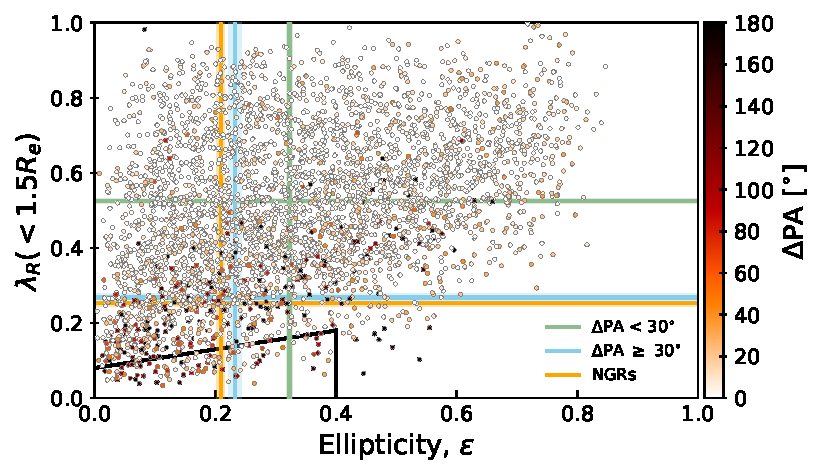
\includegraphics[width=\linewidth]{thesis/latex/misalignment_MaNGA/delPA_lambda_Re.pdf}
    \caption{$\lambda_R$ within 1.5$\mathrm{R_e}$ against ellipticity, $\epsilon$ for all galaxies with defined $\Delta$PA. The individual points are for all $\Delta$PA defined MaNGA galaxies coloured by $\Delta$PA according to the colorbar. Medians for kinematically aligned ($\Delta$PA < 30$^{\circ}$), misaligned ($\Delta$PA > 30$^{\circ}$) and NGRs are shown by the green, light blue and orange lines respectively. The lighter shade around each line corresponds to the standard error. Aligned galaxies reside more typically in the fast rotator regime with higher $\lambda_R$ and $\epsilon$, whereas misaligned galaxies and NGRs reside closer to the slow rotator regime. The same qualitative trends are found if this plot is made for ETGs, S0-Sas or Sb-Sds alone.}
    \label{fig:delPA_lambda_Re}
\end{figure}

In Figure \ref{fig:delPA_gasM} we show the distribution of gas masses for the aligned, misaligned and NGRs. We see a clear trend of lower gas mass going from kinematically aligned galaxies to misaligned galaxies to NGRs. We note that the majority ($\sim$80\%) of NGRs do not contain enough gas to have a measured gas mass from the routine of Pipe3D, so the distribution shown is a hard upper limit on the gas that these galaxies contain. We note that these trends remain qualitatively the same when considering the distributions for ETGs, S0-Sas and Sb-Sds individually.

\begin{figure}
    \centering
	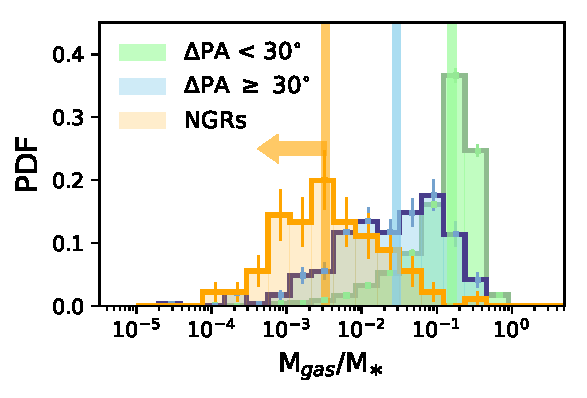
\includegraphics[width=0.8\linewidth]{misalignment_MaNGA/gas_mass_normed_all.pdf}
    \caption{Probability density distributions of gas mass fraction, $\mathrm{(M_{gas}/M_{\ast})}$ for aligned galaxies ($\Delta$PA < 30$^{\circ}$) shown in green, those with high misalignment ($\Delta$PA > 30$^{\circ}$) in light blue and NGRs in orange. Each histogram is given with Poisson errors on each bin. The vertical lines denote the corresponding distribution's median. The majority of NGRs do not have detectable gas masses and therefore the distribution shown should be considered as upper bound.}
    \label{fig:delPA_gasM}
\end{figure}

The similarity in stellar angular momentum between the NGRs and kinematically misaligned galaxies could indicate that they are from the same evolutionary sequence. A key component in decoupling star-gas rotation in simulations is a significant gas loss followed later by the accretion of material with misaligned angular momentum \citep[][]{vdvoort2015, starkenburg+19}. This gas loss can happen due to interactions from neighbouring galaxies which strips gas or through ejection due to black hole feedback.

In \red{section halo assembly} \citet{duckworth2019a}, it was shown that kinematic decoupling shows little relationship with distance to filamentary structure. This could point to stripped/ejected material being re-accreted as a potential source of misalignment between star and gas rotation. Some NGRs could therefore represent an earlier timestamp before this material is re-accreted. Not all NGRs would necessarily re-accrete gas, meaning that some would remain quenched (and hence would not become misaligned in the future) potentially explaining the differences we see in stellar mass distributions of NGRs and misaligned. In this scenario, it would suggest that re-accretion of new material does not significantly alter the stellar angular momentum content going from NGRs to misaligned.

\subsubsection{Morphology}
We now sub-divide the total population by morphology into ETGs, S0-Sas and Sb-Sds as defined in \S\ref{sec:morph_def_obs}. Figure \ref{fig:morph_PA}, shows the distributions for each category. We find that for all morphological types, galaxies are most commonly aligned with strong peaks below $\Delta$PA $\sim 30^{\circ}$. ETGs show a flatter distribution than their later counterparts, as the most likely to exhibit misalignment. LTGs show deeper drop-offs above $\Delta$PA $\sim 40^{\circ}$, with a boost around $\Delta$PA = 180$^{\circ}$, seen most strongly for the Sb-Sds. We quantify the overall misalignment fractions in the first column of Table \ref{tab:mega_table}. Our errors are estimated by binomial counting errors so that $\mathrm{\sigma = \sqrt{p(1-p) / M}}$ where $\mathrm{p = N/M}$ with $\mathrm{N}$ being the number of misaligned galaxies and $\mathrm{M}$ the total number of galaxies for the category.

This morphological difference in misalignment is likely a result of several factors. Gas rich LTGs have typically higher specific angular momentum, and hence, require a higher magnitude gas inflow/outflow with different angular momentum to disrupt rotation and create misalignment. Conversely, ETGs are more dispersion dominated and gas poor enabling smaller gas in-flows (or outflows) to create a kinematic misalignment. 

These results are reasonably consistent with previous findings of 36$\pm$5\% (of 260 galaxies) of ETGs that are misaligned in ATLAS\textsuperscript{3D} and in SAMI (45$\pm$6\% of 36 pure ellipticals, 5$\pm$1\% in 221 pure late spirals) \citep[][]{davis2011, bryant2019}. We note that our ETG misalignment fraction ($\sim$28\%) is lower than these previous findings and holds a slight tension with \citet{bryant2019}. Possible reasons for the differences may be due to morphology definition, stellar mass distribution or simply sample size. We note that enforcing stricter thresholds for morphology classifications doesn't change our misaligned fractions pointing to a likely difference in mass distributions or our increased sample size. 

\begin{table*}
\begin{tabular}{lllll}
\hline
        &  & All & Centrals & Satellites \\
\hline
All galaxies & $\Delta$PA defined &  3798 &  2185 &  1007 \\
& $\Delta$PA $\geq 30^{\circ}$ &  420 (11.1$\pm$0.5\%) &  251 (11.5$\pm$0.7\%) &  102 (10.1$\pm$1.0\%) \\
& NGR & 742 &  334 &  324 \\

ETGs & $\Delta$PA defined & 301 & 204 & 97 \\
& $\Delta$PA $\geq 30^{\circ}$ & 84 (27.9$\pm$2.6\%) & 60 (29.4$\pm$3.2\%) & 24 (24.7$\pm$4.4\%)  \\
& NGR & 231 & 140 & 91 \\

S0 - Sas & $\Delta$PA defined & 677 & 483 & 194 \\
& $\Delta$PA $\geq 30^{\circ}$ &  66 (9.7$\pm$1.1\%) & 49 (10.1$\pm$1.4\%) & 17 (8.8$\pm$2.0\%) \\
& NGR & 100 & 44 & 56 \\

Sb - Sds & $\Delta$PA defined & 1634 & 1112 & 522 \\
& $\Delta$PA $\geq 30^{\circ}$ & 88 (5.4$\pm$0.6\%) & 58 (5.2$\pm$0.7\%) & 30 (5.7$\pm$1.0\%) \\
& NGR & 107 & 32 & 75 \\

\end{tabular}
\caption{Total number of galaxies used in this study for each of $\Delta$PA defined sample, of those that are kinematically misaligned and those that have well defined stellar rotation but incoherent gas (NGR). These are defined for both splitting on morphology (rows) and group membership (columns). For those that are kinematically misaligned ($\Delta$PA $\geq 30^{\circ}$), the percentage with respect to all those with $\Delta$PA measurements for the sub-category is shown. The uncertainties quoted are binomial counting errors.}
\label{tab:mega_table}
\end{table*}

The boost in the PDF around 180$^{\circ}$ of Figure \ref{fig:morph_PA} suggests that near counter-rotation is a stable state for galaxies. This is seen most prominently in Sb-Sds with a clear upwards trend in the PDF from $\sim$140$^{\circ}$. A possible explanation is that these rotation dominated galaxies host strong stellar torques, which act to realign gas at intermediate misalignments ($30^{\circ} < \Delta$PA $ < 150^{\circ}$) on much faster timescales than in ETGs. Counter-rotators, however, remain stable and hence contribute proportionally higher to the misaligned distribution, in comparison to those at intermediate misalignments which settle towards alignment or counter-rotation.

Interestingly galaxies that exhibit near-counter rotation ($\Delta$PA $\geq$ 150$^{\circ}$) have similar stellar angular momentum to the general misaligned population ($\Delta$PA $\geq$ 30$^{\circ}$), significantly lower than the aligned counterparts. This holds true for all morphologies. \citet{chen2016} previously highlighted the boost in star formation in central regions for counter-rotating LTGs. As suggested, this could be a natural result of cancellation of angular momentum leading to increased in-flows to central regions. Our finding of lowered angular momentum in the counter-rotators (with respect to the co-rotators) supports this claim.

\begin{figure}
	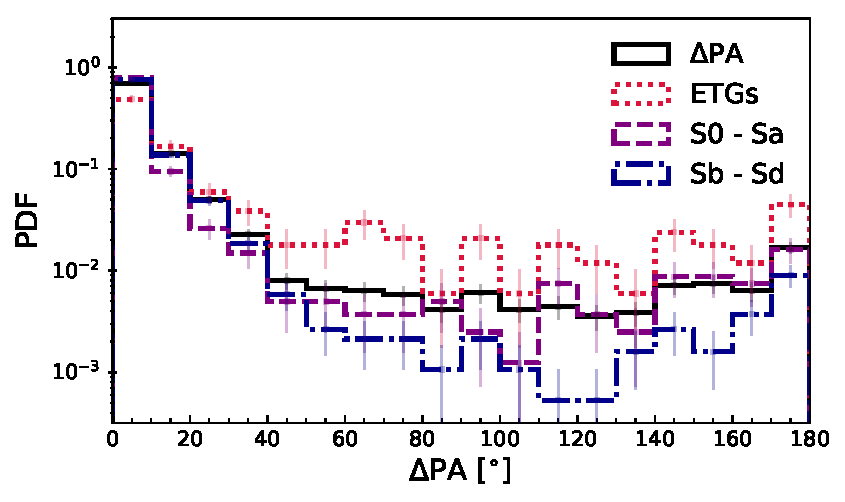
\includegraphics[width=\linewidth]{thesis/latex/misalignment_MaNGA/delPA_morph.pdf}
    \caption{Probability density distributions of kinematic misalignment as defined by $\Delta$PA split on morphology. The probability density distribution is normalised to 1 and shown in log scale. Distributions for the total population, ETGs, S0/Sa and Sb-Sds are shown by black solid, dotted red, dashed purple and dot-dashed blue lines respectively. Earlier type galaxies are more likely to be misaligned than later type galaxies.}
    \label{fig:morph_PA}
\end{figure}

Due to the relationship between stellar mass, morphology and specific angular momentum \citep[e.g.][]{cortese2016}, it might be expected that misaligned galaxies should be at higher stellar mass due to their lower $\mathrm{\lambda_{R}}$ with respect to the aligned \citep[see also;][]{bryant2019}. Surprisingly for the overall population we see little difference, however, splitting on morphology as shown in Figure \ref{fig:morph_stelM} reveals individual trends. Misaligned ETGs (and NGRs) are more massive than the aligned counterparts most likely indicative that misaligned galaxies have had richer merger histories. The opposite trends are seen for both S0-Sas and Sb-Sds with kinematically aligned galaxies being of typically higher mass than the misaligned. This could be indicative that the pathways leading to misalignment are different as a function of morphology.

\begin{figure}
    \centering
	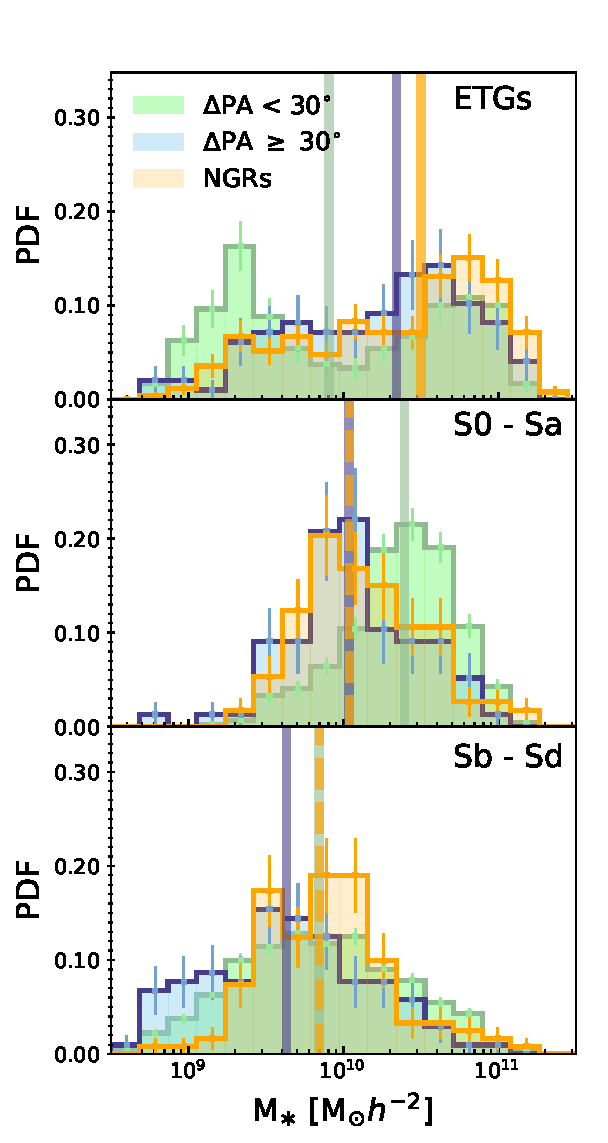
\includegraphics[width=0.5\linewidth]{thesis/latex/misalignment_MaNGA/delPA_stelM_morph_nsa.pdf}
    \caption{Probability density distributions of stellar mass, $\mathrm{(M_{\ast}/M_{\odot})}$ for aligned galaxies ($\Delta$PA < 30$^{\circ}$, misaligned galaxies ($\Delta$PA > 30$^{\circ}$) and NGRs for ETGs, S0-Sas and Sb-Sds (top to bottom). In each panel the aligned/misaligned are shown with solid lines with the aligned in the darker shade. NGRS are shown by dot-dashed lines. Each histogram is given with Poisson errors on each bin. The vertical lines denote the corresponding distribution's median. For ETGs, aligned galaxies are less massive than the misaligned sample. This trend, however, reverses for S0-Sas and Sb-Sds.}
    \label{fig:morph_stelM}
\end{figure}

\subsubsection{Group membership}
Group membership is important for dictating the evolution of a galaxy and hence we now sub-divide our population into centrals and satellites as described in \S\ref{sec:group_def}. Figure \ref{fig:group_morph_PA} (top panels) shows the $\Delta$PA distributions as in Figure \ref{fig:morph_PA}, but now split into centrals and satellites. Qualitatively the morphological trends remain however Table \ref{tab:mega_table} reveals that centrals (29.4$\pm$3.2\%) are slightly more likely to be misaligned than satellites (24.7$\pm$4.4\%) for ETGs. This is also potentially seen for the S0-Sbs (10.1$\pm$1.4\% for centrals vs 8.8$\pm$2.0\% for satellites), however we note that both fractions are within each other's errorbars.

\begin{figure*}
    \centering
	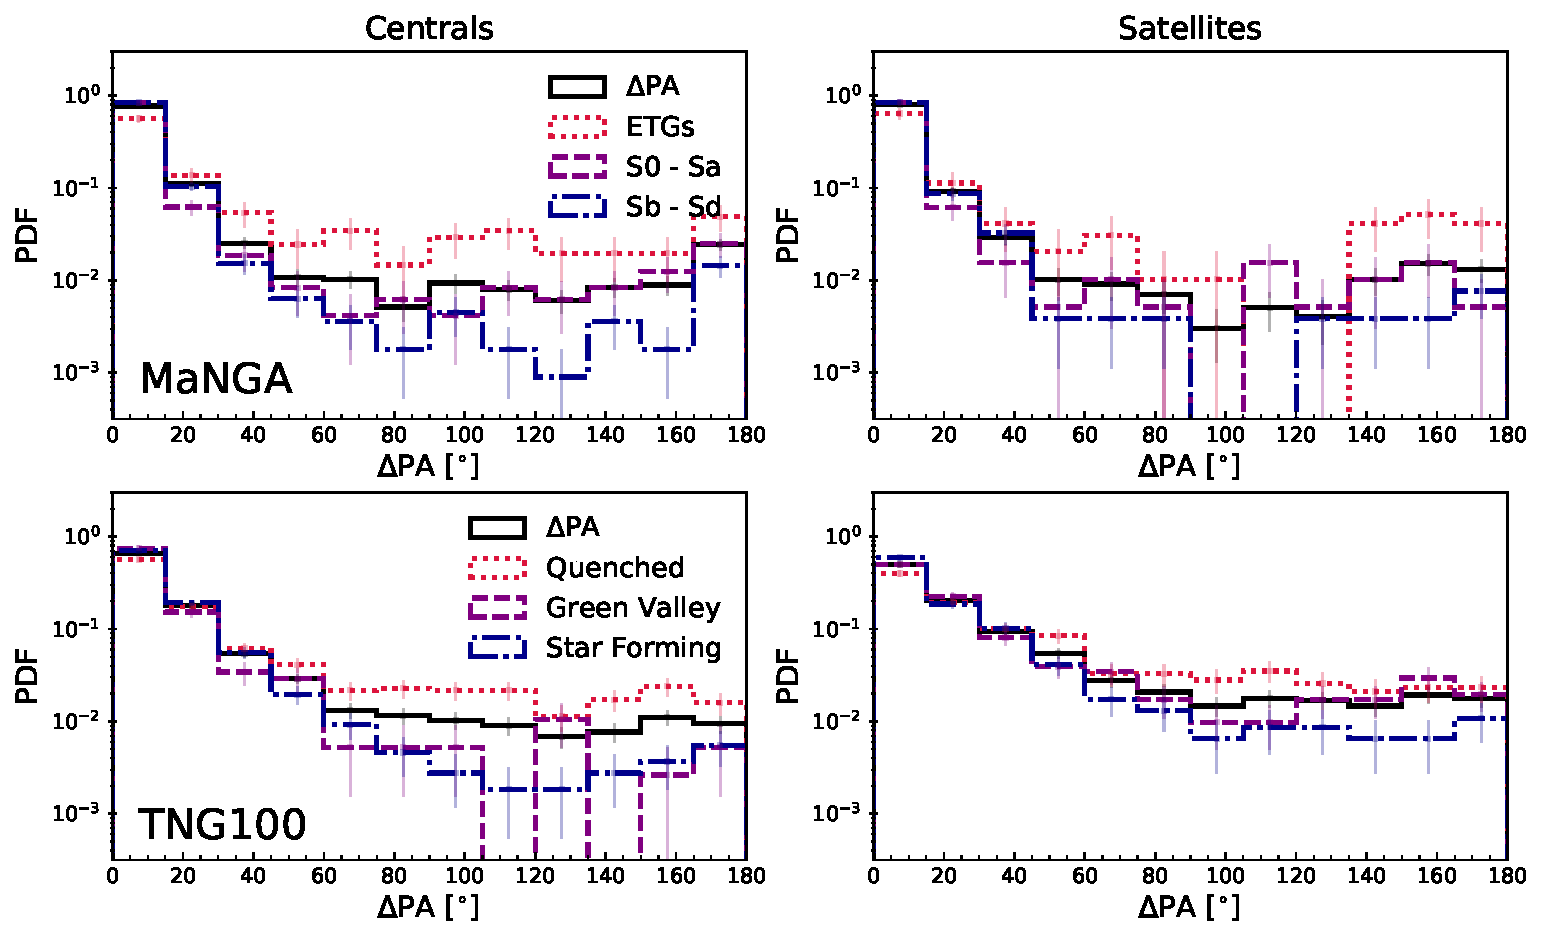
\includegraphics[width=\linewidth]{misalignment_MaNGA/MPL8_TNG_morph_group_PA.pdf}
    \caption{Same as Figure \ref{fig:morph_PA}, however split by group membership into centrals (left) and satellites (right). The top panel shows for the MaNGA sample and the bottom shows for the mock sample in TNG100. Morphology for TNG100 is categorised by the deviation of the galaxy's star formation away from the main sequence of galaxies in the whole of TNG100 (see \S\ref{sec:tng_results})}
    \label{fig:group_morph_PA}
\end{figure*}

Figure \ref{fig:group_morph_stelM} shows the stellar mass distribution for our samples but now additionally split into centrals and satellites. Again we find the same qualitative trends for both centrals and satellites; i.e. misaligned ETGs are more massive than their aligned counterparts whereas misaligned S0-Sas and Sb-Sds are less massive than those aligned.
\begin{figure*}
    \centering
	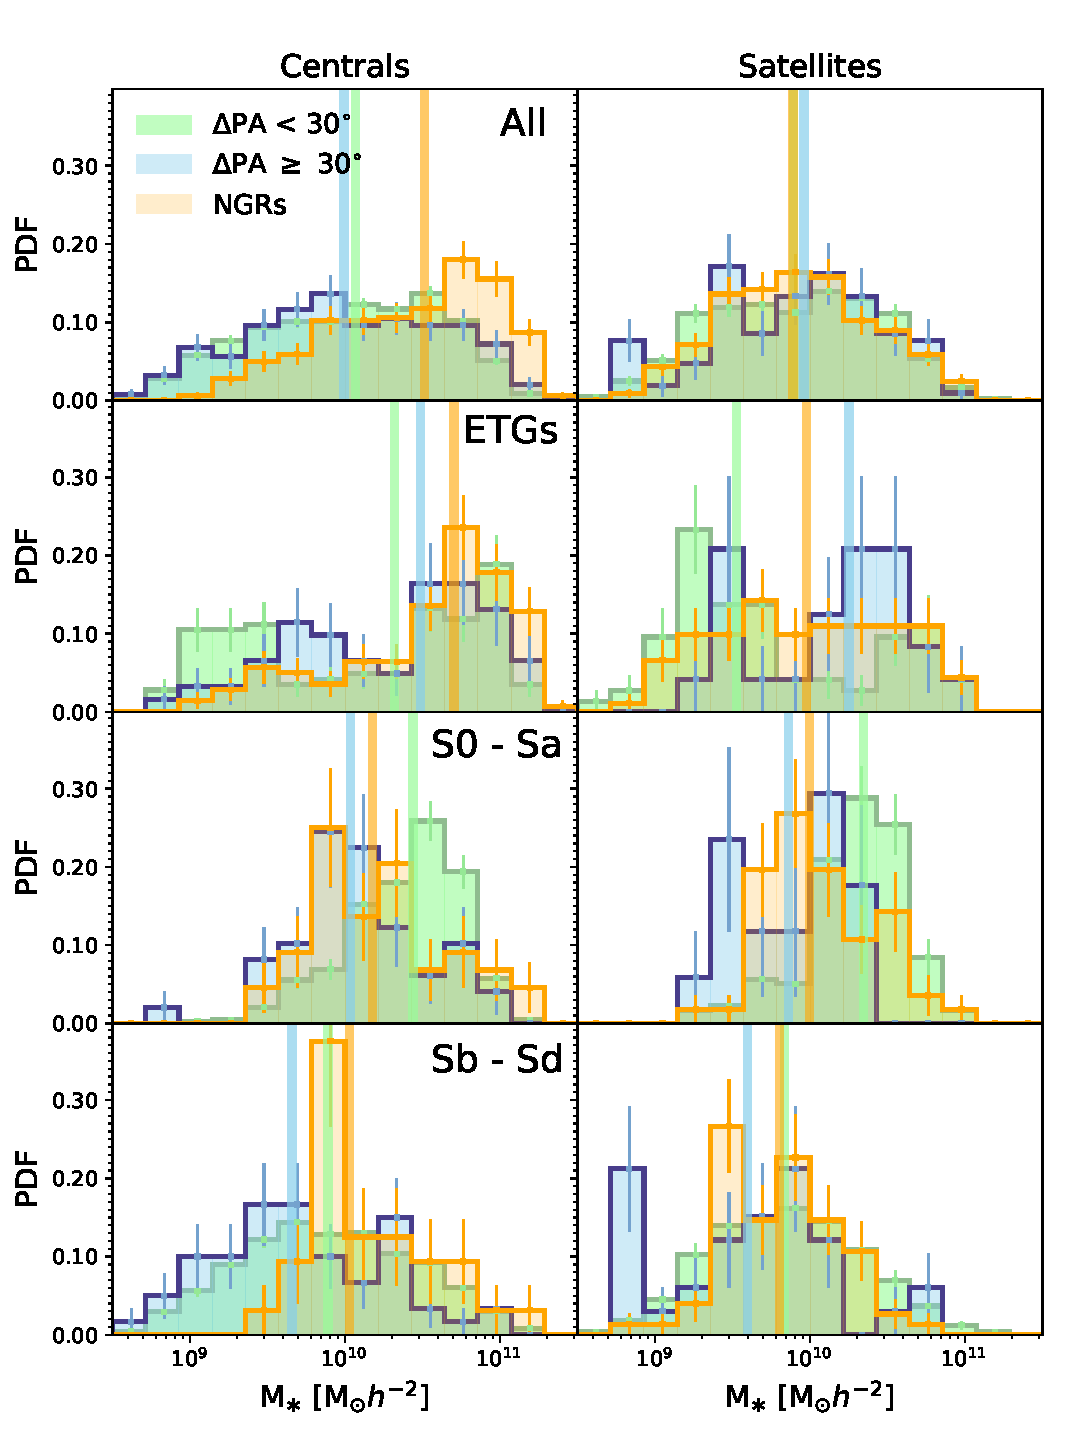
\includegraphics[width=0.85\linewidth]{misalignment_MaNGA/delPA_stelM_morph_lim_nsa.pdf}
    \caption{Same as Figure \ref{fig:morph_stelM}, however split by group membership into centrals (left) and satellites (right). Additionally the distributions for the overall central and satellite populations is shown in the top row. We see that for ETGs there is a strong difference in mass between aligned and misaligned satellites. This trend is reversed for S0/Sa and Sb/Sd satellites. These trends are also seen for centrals, however, typically to a lesser degree.}
    \label{fig:group_morph_stelM}
\end{figure*}

\subsection{Summary of observations} \label{sec:summary_manga}
In this chapter, we introduce a catalogue of $\sim$4500 galaxies from the MaNGA survey in order to establish the
prevalence of misalignment as a function of optical morphology. We also relate the typical stellar angular momentum and gas content of kinematically misaligned galaxies relative to the aligned. Our conclusions are as follows:

\begin{enumerate}
    \item The prevalence of kinematic misalignment (i.e. where rotational axes of stars and gas are offset by $> 30^{\circ}$) is strongly morphological dependent with ETGs having $\sim$28\% exhibiting misalignment which decreases to $\sim$5\% for Sb-Sds.
    
    \item For all morphologies this misalignment is related to a lowered stellar angular momentum and also a lowered gas mass. We note that misaligned galaxies have similar stellar angular momentum to those do not have coherently rotating gas (those with large gas depletion fall into this category). This could be indicative that galaxies without coherent gas rotation and kinematically misaligned galaxies are different timesteps in the same evolutionary sequence. As noted in simulations \citep[][]{vdvoort2015, starkenburg+19}, a key component in decoupling star-gas rotation is a significant gas loss followed by accretion of new gas with misaligned angular momentum. In this scenario, NGRs could represent an earlier timestamp before a future re-accretion of gas. This would indicate that the stellar angular momentum is disrupted prior to accretion of new material. 
    
    \item We find that the misalignment fraction is also dependent on group membership. For ETGs and S0-Sas, central galaxies are more likely to exhibit misalignment than satellites. For Sb-Sds this trend reverses.
    
    \item We find that counter-rotation (i.e. rotational axes of stars and gas are offset by $> 150^{\circ}$) is a stable state for galaxies of all morphologies shown by a boost in the PDF (Figure \ref{fig:morph_PA}). Similar to the total misaligned population, counter-rotators have distinctly lower angular momentum than their aligned counterparts. 

\end{enumerate}
In the following section, we investigate whether hydrodynamical simulations can reproduce these observed trends and what typical timescales are associated with angular momentum and gas loss.

\section{In IllustrisTNG} \label{sec:tng_kin_mis}
\subsection{Simulation data} \label{sec:sim_data_TNG}
\subsubsection{IllustrisTNG} 
The IllustrisTNG project \citep{marinacci18,naiman18,nelson18,pillepich18b,springel18} is a suite of magneto-hydrodynamic cosmological scale simulations incorporating an updated comprehensive model for galaxy formation physics \citep[as decribed in][]{weinberger17,pillepich18a} and making use of the moving-mesh code \texttt{AREPO} \citep{springel10,pakmor11,pakmor13}. For this work, we use the highest resolution fiducial run of TNG100 which follows the evolution of 2 x 1820$^3$ resolution elements within a periodic cube with box lengths of 110.7 Mpc (75 h$^{-1}$ Mpc). This corresponds to an average mass resolution of baryonic elements of 1.4 x 10$^6 \mathrm{M_{\odot}}$ and 7.5 x 10$^6 \mathrm{M_{\odot}}$ for dark matter. Here we make use of public data from the IllustrisTNG project \citep[as described in][]{nelson2019}.

Structure in TNG100 is identified into haloes and subhaloes as follows. Haloes (also referred to as FoF haloes or Groups) are found from a standard friends-of-friends (FoF) algorithm \citep{davis85} with linking length $b=0.2$. The FoF algorithm is run on the dark matter particles, and the other types (gas, stars, BHs) are attached to the same groups as their nearest DM particle. Each halo is then divided into gravitationally bound subhaloes through the subfind algorithm \citep{springel01}. In short, subfind defines `subhaloes' as locally over-dense and self-bound particle groups as distinct objects within given FoF haloes. We consider all subhaloes at $z=0$ containing a minimum stellar mass of $\mathrm{M_{\ast}} = 10^{8.5} \mathrm{M_{\odot}}$ to potentially make up our mock MaNGA like sample. Since we are typically considering the stellar component of these subhaloes for our mock observations, we will refer to these as TNG100 galaxies.

\subsubsection{Matching to MaNGA sample}
To construct a mock MaNGA sample we select representative subhaloes from TNG100. For every MaNGA galaxy, we find the TNG100 galaxy with the most similar stellar mass, size and SDSS $g - r$ colour. In this instance, stellar mass is defined by the total mass of stellar particles within a radius of 2 stellar effective radii. The SDSS $g - r$ colour is found using the prescription outlined in \citet{nelson18}. Here we describe the general process, while we direct the reader to \citet{nelson18} for more detail. Each stellar particle in the simulation is modelled as a single-burst simple stellar population. This is converted into a population spectrum using FSPS \citep{conroy2009,conroy2010,foreman_mackey2014} which is convolved with the pass-bands for SDSS colours. We use model C \citep[as described in][]{nelson18} which also includes models for unresolved and resolved dust. We use sizes following the prescription of \citet{genel2018}, which use a projected half light radius. The SDSS bands are constructed as above and are used to define circular half light radii for each SDSS band along X, Y and Z projections of the box. We use the $r-$band half light radius projected perpendicular to the XY plane, consistent with the line of sight of the mock MaNGA observation.

The matching is done through finding the closest neighbour in a normalised space with dimensions of the matched properties. If multiple MaNGA objects match to a given TNG100 galaxy then the absolute nearest neighbour is selected and the MaNGA object is assigned to its second nearest neighbour. The process is iterated until all have unique matches. 

The galaxy is then assigned the same bundle size IFU as the matched MaNGA galaxy with the corresponding angular resolution. The galaxy is then `observed' (see \S\ref{sec:mock_obs}) at a distance so that the angular footprint of the assigned IFU covers the same number of physical effective radii for the mock galaxy as the matched observation. 

\subsubsection{Mock observations} \label{sec:mock_obs}
We convert each galaxy in TNG100 into a mock MaNGA observation, as follows:

We take the raw particle/cell data of gas and stars and project on the XY plane (i.e. z-direction is the line of sight). Since there is no preferred direction in the simulation, this corresponds to a `random' viewing angle of each galaxy. We bin particles corresponding to the angular resolution of spaxels in MaNGA (0.5 arcsec/pixel), in the distinct hexagonal footprint of MaNGA observations. In each bin, we calculate the mean velocity, velocity dispersion and total flux for all particles. 

Since we include all particles along the line of sight, we must take care in interpreting the absolute values of flux, since none is lost due to obscuration. We, however, do not use the flux values calculated here in our work.

In order to estimate the typical noise associated with a MaNGA observation, we compute radial profiles of the signal to noise ratio (SNR) for all MaNGA observations of a given IFU size. MaNGA has 5 different IFU sizes corresponding to bundles of 19, 37, 61, 91 and 127 fibres. MaNGA provides estimates of the SNR for every spaxel in each observation in the $g$-band. Figure \ref{fig:noise_profile} shows the azimuthally averaged SNR profiles for all MaNGA observations of each fibre bundle size. We fit a logarithmic function to each profile, which is used to assign noise to the mock observations. Noise is drawn for each pixel from a normal distribution using the median and standard deviation of the fitted logarithmic radial profile.

\begin{figure}
    \centering
	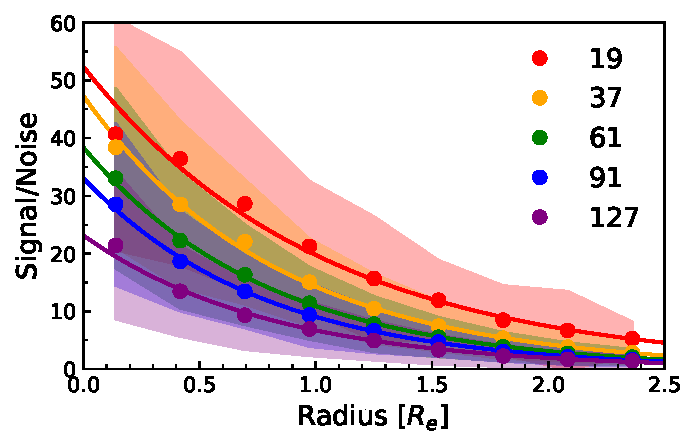
\includegraphics[width=0.95\linewidth]{misalignment_TNG/noise_profiles_ifusize.pdf}
    \caption{Average signal to noise profiles for each IFU size for all MaNGA MPL-8 observations. The circles show the median value for each radius bin with the shaded region corresponding to the standard deviation. The solid line corresponds to an logarithmic parametric fit to the data points, used in sampling the noise profile for the mock observations.}
    \label{fig:noise_profile}
\end{figure}

In order to simulate the effects of the point spread function (PSF), we then convolve our binned particle data with a Gaussian kernel. MaNGA observations typically have a $g$-band PSF which can be fit with a Gaussian of $\sim 2-3''$ full width half maximum (FWHM). We take all our mock observations to have a PSF modelled by a Gaussian with a 2$''$ FWHM. The spatial scale of the simulation is effectively set by the gravitational softening length of both the DM and stellar particles at 0.5h$^{-1}$ kpc = 0.74 kpc. This is approximately a factor of two (four) lower than the spatial sampling (PSF) of a typical MaNGA observation. The typical spatial resolution of star forming gas cells in TNG100 is of order $\sim$200pc and therefore suitable for our mock observations. We direct the reader to Figure 1 in \citet{pillepich2019} for further details (scale by a factor of $16^{1/3}$ for TNG100). \red{Do you direct readers elsewhere for a thesis?}

We fit position angles to MaNGA observations that have been Voronoi binned so that bins contain a minimum S/N $\sim 10$. To maintain consistency and avoid spurious individual particles biasing measurements, we also Voronoi bin our mock observations so that a minimum of 5 particles is contained within a given bin, again using the routine of \citet{cappellari2003}. Figure \ref{fig:example_obs} shows example stellar (and gas) velocity and dispersion fields along with normalised $r$-band flux, after our processing.

\begin{figure*}
	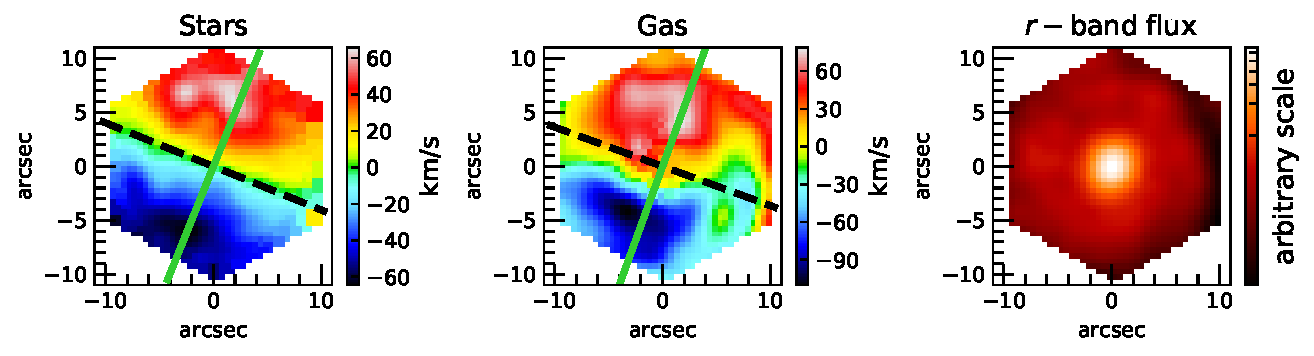
\includegraphics[width=\linewidth]{misalignment_TNG/example_kinematics.pdf}
    \caption{Example outputs from a MaNGA-like observation in TNG100. Shown (left to right) are the stellar velocity field, gas velocity field and normalised $r-$band flux for a given galaxy, `observed' under the same conditions of its MaNGA counterpart (i.e. distance and IFU size). For the stellar and gas velocity fields, the kinematic PA fits (see \S\ref{sec:def_kin_mis}) are shown (green solid line) with the axis of rotation (black dotted line).}
    \label{fig:example_obs}
\end{figure*}

\subsection{Comparisons to observations} \label{sec:manga_tng_comp}
\subsubsection{$\Delta$PA}
Firstly we consider all $\Delta$PA defined galaxies for both MaNGA and TNG100. Figure \ref{fig:total_pa_dist} shows the distribution of $\Delta$PA for both MaNGA and IllustrisTNG100. Both distributions are strongly peaked around around 0$^{\circ}$ indicative of the preferentially aligned state predicted from tidal torquing theory. The MaNGA distribution shows a sharp drop-off past 40$^{\circ}$ whereas TNG100 shows a smoother drop off to higher misalignments. Additionally the MaNGA distribution shows a second peak around 180$^{\circ}$ indicative of the stable counter-rotating state identified in previous work \citep[e.g.][]{chen2016}. This secondary peak is not seen for the overall TNG100 sample, however is apparent for star forming galaxies in TNG100 (see bottom panel of Figure \ref{fig:group_morph_PA}). 

\begin{figure}
    \centering
	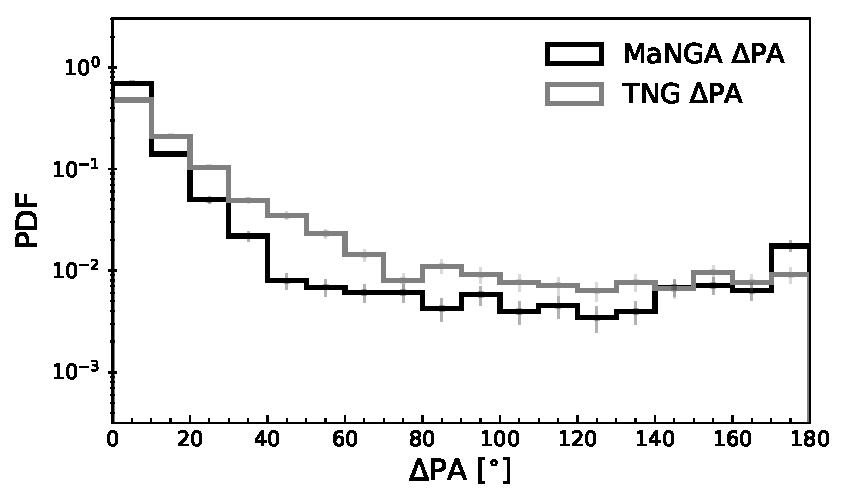
\includegraphics[width=0.85\linewidth]{misalignment_TNG/mpl8_pa_dist.pdf}
    \caption{Probability density distribution of kinematic misalignment as defined by $\Delta$PA for the total MaNGA sample (black line) and matched TNG100 sample (grey line). $\Delta$PA is strongly peaked around 0$^{\circ}$ with a small boost close to 180$^{\circ}$.}
    \label{fig:total_pa_dist}
\end{figure}

The TNG100 mock sample reproduces the general trends well, when considering the differences in how we split the samples in observations and simulations. The smoother drop-off past 40$^{\circ}$ for TNG100 is likely a combination of how we construct the mock observations and scatter in the mass distributions between the MaNGA and TNG100 samples. By construction the matching between MaNGA and TNG100 objects is done before $\Delta$PA is calculated. For this reason there may be differences between the mass distribution of the $\Delta$PA defined MaNGA and TNG100 samples, as shown in Figure \ref{fig:TNG_mpl8_stelM}. We find that the misaligned sample in TNG100 is slightly more massive with respect to MaNGA whereas the aligned samples are consistent. Due to the strong morphological dependence on kinematic misalignment, there is a secondary dependence on stellar mass. The increased overall fraction of misaligned galaxies in TNG100 is therefore, in part, due to the TNG100 $\Delta$PA defined sample being slightly more massive. This slight boost could indicate that the mechanisms for misalignment may be different in simulations than observations. \citet{khim2019} compare the misalignment fractions in observations (SAMI) with simulations (Horizon-AGN). While overall a good agreement is found, they note a significant difference in cluster environments where simulated galaxies are far more likely to be misaligned than in observations. More work needs to be done to understand how well cosmological hydrodynamical simulations replicate the processes leading to misalignment in observations, however, overall trends appear to be well reproduced for different simulation prescriptions.

\begin{figure}
    \centering
	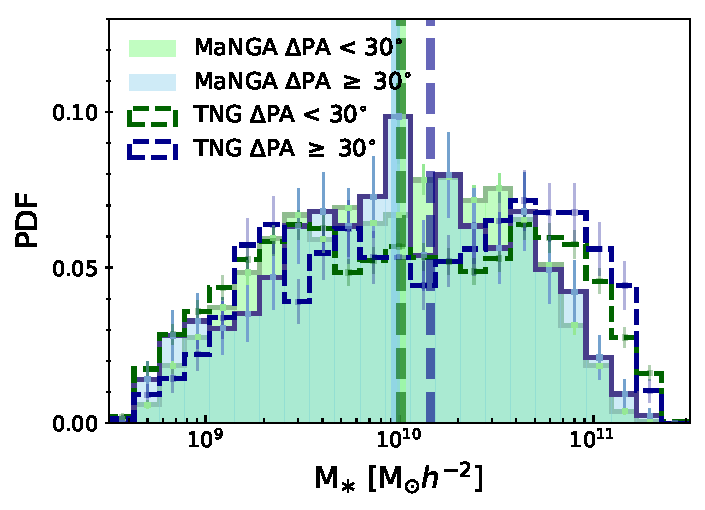
\includegraphics[width=0.85\linewidth]{misalignment_TNG/delPA_split_stelM_tng_comparison.pdf}
    \caption{Probability density distributions of stellar mass, $\mathrm{(M_{\ast}/M_{\odot})}$ for aligned galaxies ($\Delta$PA < 30$^{\circ}$, green) and misaligned galaxies ($\Delta$PA > 30$^{\circ}$, red) defined in MPL-8 (solid lines) and TNG100 (dashed). The vertical lines denote the corresponding distribution's median. The overall distributions are a reasonable match between mocks and observations, with a noted preference for $\Delta$PA defined galaxies at the very high mass end for TNG100. }
    \label{fig:TNG_mpl8_stelM}
\end{figure}

\subsubsection{Morphological dependence} 
We divide our mock MaNGA sample based on the instantaneous star formation rate (SFR) of the galaxy. Here, we define SFR for all gas cells within twice the stellar half mass radius of a given galaxy. The star forming main sequence for all galaxies is found by fitting a power law as a function of stellar mass. A galaxy is then flagged into one of three categories; star forming, green valley or quenched depending on its deviation above or below the main sequence \citep{pillepich2019}. The selected deviations from the main sequence are as follows; star forming galaxy: $\mathrm{\Delta \log_{10}(SFR) > −0.5}$, green valley galaxy: $\mathrm{-1.0 < \Delta \log_{10}(SFR) < -0.5}$ and quenched galaxy: $\mathrm{\Delta \log_{10}(SFR) <= -1.0}$. \red{check this.}

The bottom panel of Figure \ref{fig:group_morph_PA}, shows the $\Delta$PA distribution for the TNG100 sample split into centrals and satellites. Comparing to the observational sample in the top panel of Figure \ref{fig:group_morph_PA}, the morphological trends remain qualitatively the same with quenched/ETGs (star forming/LTGs) more likely to be misaligned (aligned).

Our choice to compare populations split on visual morphology in observations to SFR in simulations is one of necessity. The aim of this work is to explore the relationship of visual morphology with decoupled rotation. Unfortunately we don't currently have the equivalent classifications in IllustrisTNG100, so use an appropriate proxy. In future work, we will look at the relationship between observations and simulations using machine learning classifications of morphology, however, in the following subsections we follow the evolutionary history of the mock sample split by sSFR.

\subsection{Evolution of angular momentum} \label{sec:tng_ang_mom_evo}
\subsubsection{Magnitudes}
\red{add more introduction / why you are talking about angular momentum now.}
In this section, we consider the angular momentum content of our TNG100 mock sample back to $z=1$ for stars, gas and dark matter individually. The prior time evolution such properties for each galaxy is followed by considering the main progenitor branch (most massive defined by stellar mass) in the sublink merger trees \citep{rgomez2015}. Angular momentum for our TNG100 galaxies is defined by the intrinsic specific angular momentum of their particles/cells:
\begin{equation}
\mathrm{j_{k} = \frac{1}{\sum_{n} m^{(n)}} \sum_{n} m^{(n)}\boldsymbol{x}^{(n)} \times \boldsymbol{v}^{(n)}}
\end{equation}
where $\boldsymbol{v}^{(n)}$ is the velocity of each particle relative to the centre of mass for the galaxy. $\boldsymbol{x}^{(n)}$ is the position of a given particle with respect to the position of the most gravitationally bound particle in the galaxy. We choose this definition since the centre of mass velocity can be biased by structure at large radii in the subhalo/galaxy and hence may spuriously not represent the true rotational centre. $k$ is the particle/cell type referring to either stars, gas or dark matter. For stars and gas this is calculated within a 3D radius equal to the 2D radius corresponding to the angular size of the mock observation. Dark matter is calculated for all particles assigned to the subhalo by the subfind algorithm. 

Figure \ref{fig:sJ_evo} shows the specific angular momentum evolution from $z=1$ for each of stars, gas and DM split on group membership and morphology. We see that similar to the observational sample (see \S\ref{sec:manga_total_pop}), misaligned galaxies in simulations are significantly lower stellar angular momentum than their aligned counterparts at $z=0$. This is reflected in for each of stars, gas and DM to various degrees for all morphologies and central/satellite definition. Interestingly, while misalignment between stars and gas may itself be a transient property, those misaligned at $z = 0$ reside in dark matter haloes with \textit{fundamentally lower angular momentum} which persists to at least $z = 1$. 

\begin{figure*}
	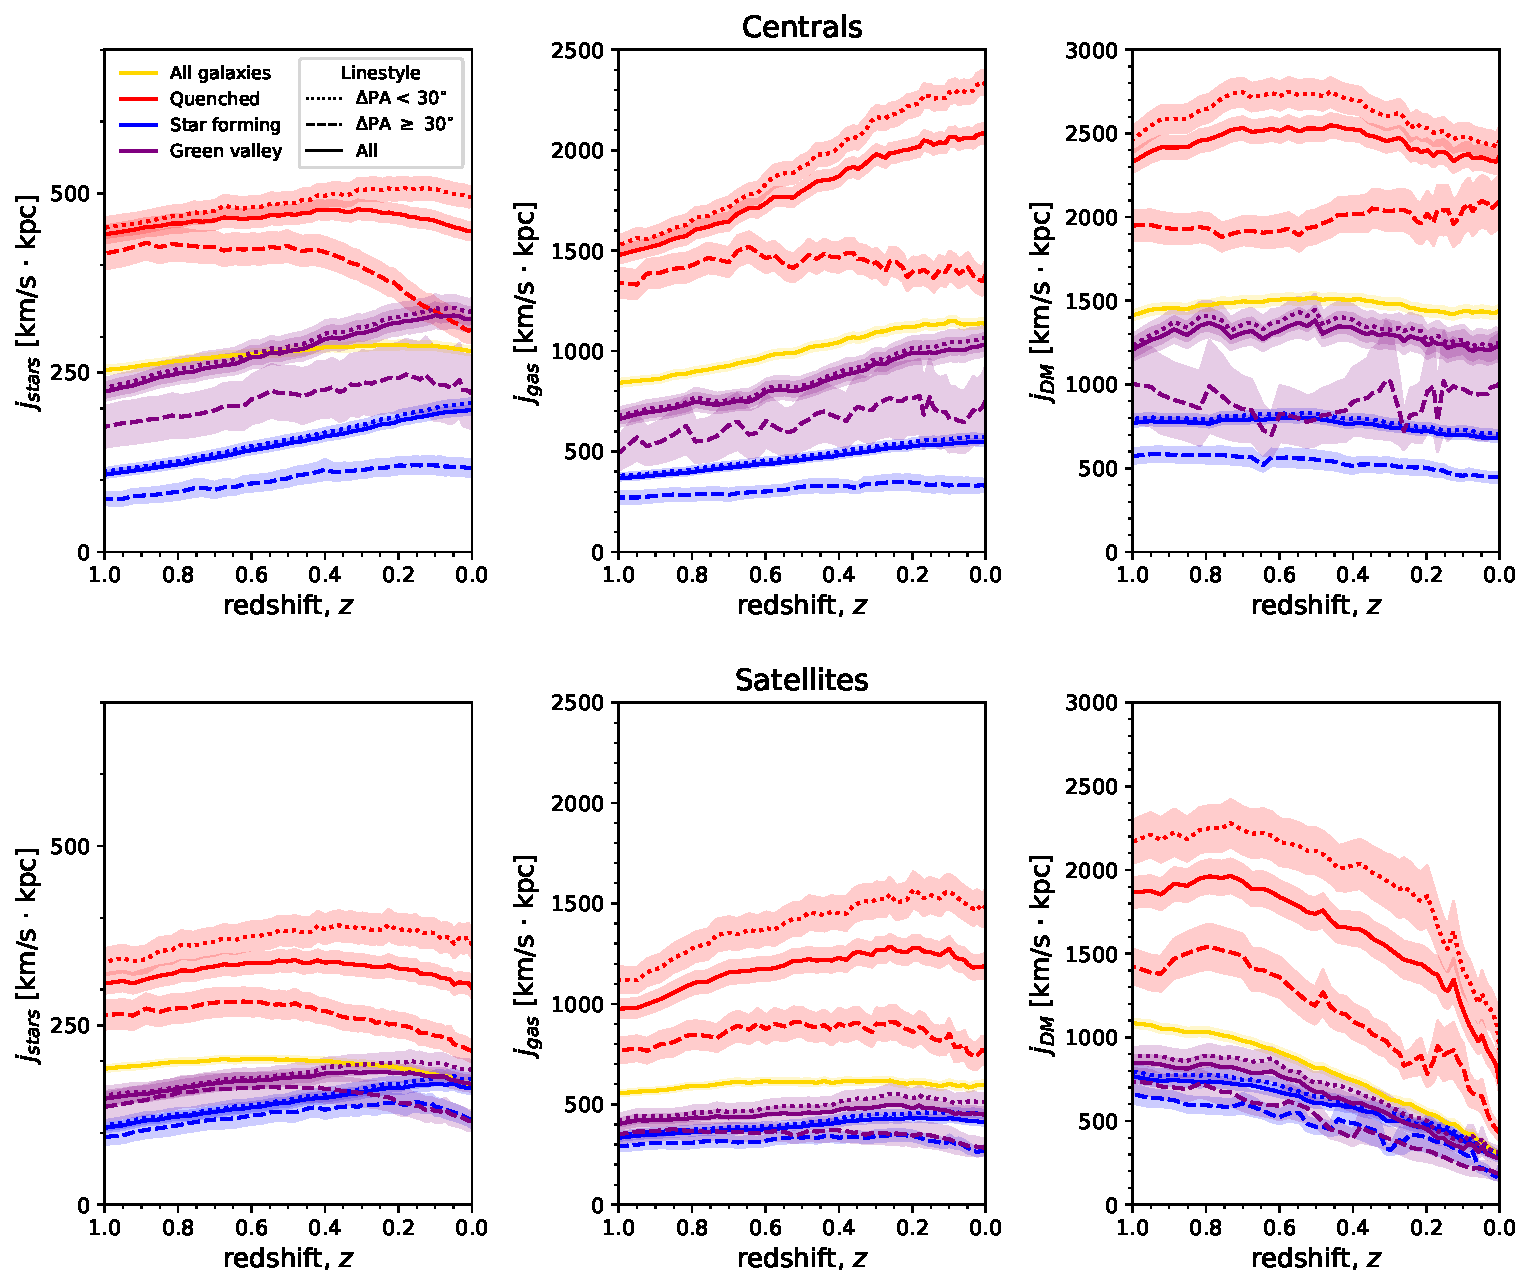
\includegraphics[width=\linewidth]{misalignment_TNG/sJ_evo_cen_sat.pdf}
    \caption{Specific angular momentum evolution from $z = 1$ calculated from star, gas and DM particles (left to right). The angular momentum is calculated for all star and gas particles/cells within the 3D radius assigned by the mock IFU observation, whereas DM is found from all particles associated to the subhalo. The evolution is taken as the median at each timestep for all galaxies of that category with errorbars showing the standard error. The top (bottom) row shows the evolution for central (satellite) galaxies. Each panel displays the evolution split into morphologies; quenched (red), green valley (purple) and star forming (blue) and also $\Delta$PA $< 30^{\circ}$ (dotted) and $> 30^{\circ}$ (dashed). Kinematically misaligned galaxies selected at $z=0$ have notably lower specific angular momentum for all of stars, gas and dark matter.}
    \label{fig:sJ_evo}
\end{figure*}

We note that particle based calculations of specific angular momentum scales with the number of particles. This results in more massive galaxies having higher $\mathrm{j_{i}}$ and further, quenched galaxies (that are typically more massive) having higher $\mathrm{j_{i}}$ than their later type counterparts. While there is only a small difference in-between the mass distributions of our aligned and misaligned samples, to ensure our signal is not simply driven by mass we calculate the residuals of $\mathrm{j_{star}}$ with respect to a typical galaxy of that mass. The residuals, $\Delta \mathrm{j_{star}}$ are calculated by fitting a polynomial to the distribution of $\mathrm{j_{star}}$ vs $\mathrm{M_{\ast}}$ for the galaxies (all mock observations, regardless if $\Delta$PA is well defined) at each snapshot. $\Delta \mathrm{j_{star}}$, is then defined as the deviation of a given galaxy away from the expectation of the fitted line at that mass. Since the trends are qualitatively consistent regardless of morphology, Figure \ref{fig:sJ_evo_residual} shows the specific angular momentum residuals for the total population. For completeness we also include comparison to every galaxy in the mock sample (regardless if $\Delta$PA is well defined). Misaligned galaxies ($\Delta$PA $\geq 30^{\circ}$) for both centrals and satellites show intrinsically lower $\Delta \mathrm{j_{star}}$ with respect to the total population at a given mass, indicative that it is not an effect due to mass. In addition, there is a relative evolution where $\Delta \mathrm{j_{stars}}$ diverges from all galaxies at $z \sim 0.5$ so that misaligned galaxies have even lower stellar angular momentum with respect to the aligned galaxies in recent times.

\begin{figure*}
	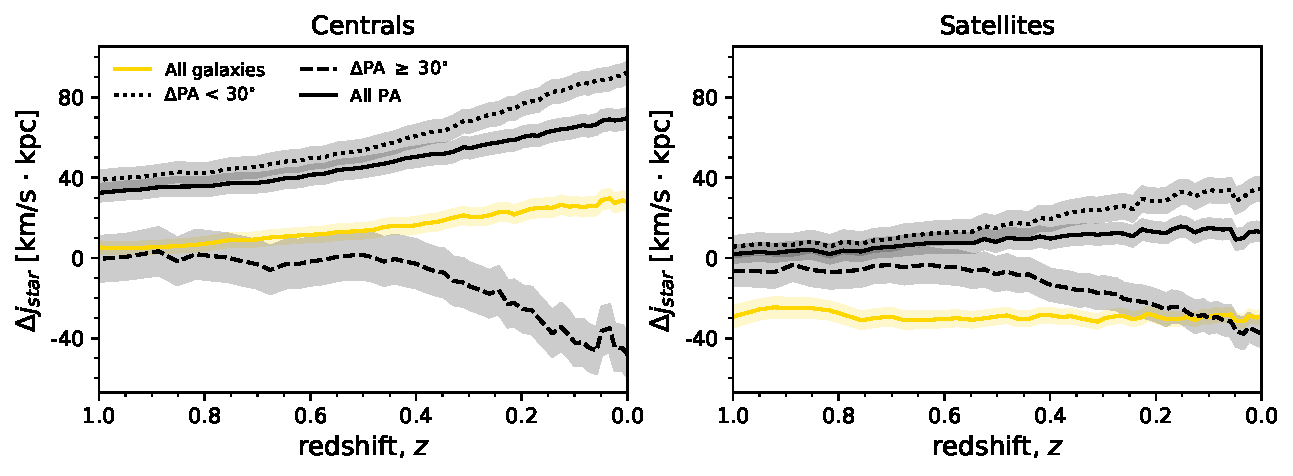
\includegraphics[width=\linewidth]{misalignment_TNG/delta_j_stars_residuals.pdf}
    \caption{The specific angular momentum residuals from $z=1$ for all star particles within the 3D radius assigned by the mock IFU observation. The residual is calculated as the deviation away from the expectation for a galaxy of that mass at each snapshot. The evolution of the residual is taken as the median at each timestep for all galaxies of that category with errorbars showing the standard error. The right (left) panel shows the evolution for central (satellite) galaxies. Each panel displays the evolution for all galaxies (yellow), of which have a defined $\Delta$PA (black solid), aligned galaxies $\Delta$PA $< 30^{\circ}$ (black dotted) and misaligned $> 30^{\circ}$ (black dashed). We see that the difference in angular momentum between aligned and misaligned galaxies is not due to differences in mass. In addition we note a marked deviation of misaligned galaxies to even lower angular momentum in recent times.}
    \label{fig:sJ_evo_residual}
\end{figure*}

\subsubsection{Direction}
\subsubsection{Computation of 3D angles and comparison to $\Delta$PA}
To conclude this section we now consider the directional 3D offsets between the angular momentum vectors of the stars, gas and dark matter. These are calculated from:
\begin{equation} \label{eq:alpha}
\mathrm{\alpha_{3D} = \text{arccos} \left( \frac{\boldsymbol{j_{i}} \cdot \boldsymbol{j_{j}}}{\left| \boldsymbol{j_{i}} \right| \left| \boldsymbol{j_{j}} \right|} \right),}
\end{equation}
where $i, j$ refer to either stars, gas or dark matter. As for the magnitudes of angular momentum, the star and gas vectors are calculated within a 3D radius set to that of the IFU footprint and the dark matter vector is calculated for all particles assigned to the subhalo by subfind.

A key assumption of this work is the ability for the projected $\Delta$PA to be a reliable estimator of the actual 3D offset between star and gas rotation axes. Figure \ref{fig:PA_residual} shows the distributions of the difference between $\Delta$PA and the 2D and 3D offsets between the angular momentum principal axes of stars and gas. See equation \ref{eq:alpha} for calculation of the 3D offset; the 2D equivalent is simply a projection of this onto the XY plane. $\Delta$PA is a reasonable measure of the true 3D offset which can be modelled as a Gaussian centred on 0$^{\circ}$ with a standard deviation of 17.6$^{\circ}$ (green dotted line). The deviation of the 2D projection from the true 3D offset (black line) has a standard deviation of 13$^{\circ}$, demonstrating that the variation is both due to projection and the noise associated with observations. Additionally, we note the different particle selection for the two measures which may drive slight differences. While the 2D/3D offsets and $\Delta$PA are measured in a footprint with the same radius, the offsets are only defined for particles within a 3D sphere of this radius, where $\Delta$PA is defined for all particles along the line of sight enclosed by the sky footprint. 

\begin{figure}
    \centering
	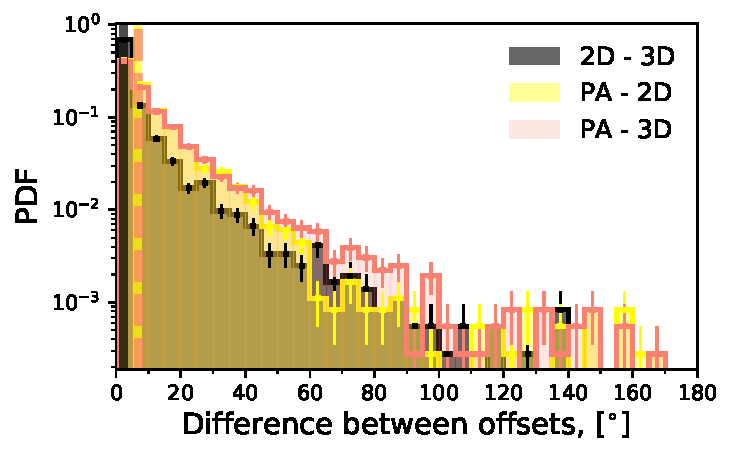
\includegraphics[width=0.9\linewidth]{misalignment_TNG/PA_alpha_resid_hist.pdf}
    \caption{Probability density distribution of the difference between various measures of the star-gas rotational angle offset. The difference between the 3D angular momentum vectors and projection in 2D is shown (black), $\Delta$PA and 2D (yellow) and $\Delta$PA and 3D (red).}
    \label{fig:PA_residual}
\end{figure}

\subsubsection{Results}
Figure \ref{fig:3D_alpha_evo} shows the evolution of the 3D offsets between each of stars, gas and DM respectively. As expected splitting our sample on $\Delta$PA results in significantly higher $\mathrm{\alpha_{STARS - GAS}}$ at $z = 0$ for the misaligned galaxies found in the MaNGA observations. This is also typically correlated, albeit less strongly, with larger $\mathrm{\alpha_{STARS - DM}}$ and $\mathrm{\alpha_{GAS - DM}}$ at $z=0$. This is indicative that a decoupling between stars and gas is often mirrored by a decoupling between the rotation of stars and DM. We also plot the average decoupling for all galaxies (all that are matched to MaNGA) between all components. In the middle panel, we see that $\mathrm{\alpha_{STARS - DM} \sim 50^{\circ}}$ on average for all galaxies (gold line) with a slight redshift evolution which is roughly consistent with previous work \citep[e.g.][]{chisari+17}. We note that our choice to consider the direction of the star and gas rotation within the observational footprint is typically far smaller than the overall DM halo, and hence, may lead to slightly higher typical misalignments between baryonic and DM components.

Working back from $z=0$, we note that $\mathrm{\alpha_{STARS - GAS}}$ for the aligned and misaligned samples (selected at $z=0$) converges in the majority of cases before $z=1$. This indicates the transient nature of misalignment. This is in stark contrast to the magnitude of angular momentum for individual components (stars, gas, DM) which show a persistent difference in magnitude between aligned and misaligned objects (selected at $z=0$) going back past at least $z=1$. 

\begin{figure*}
	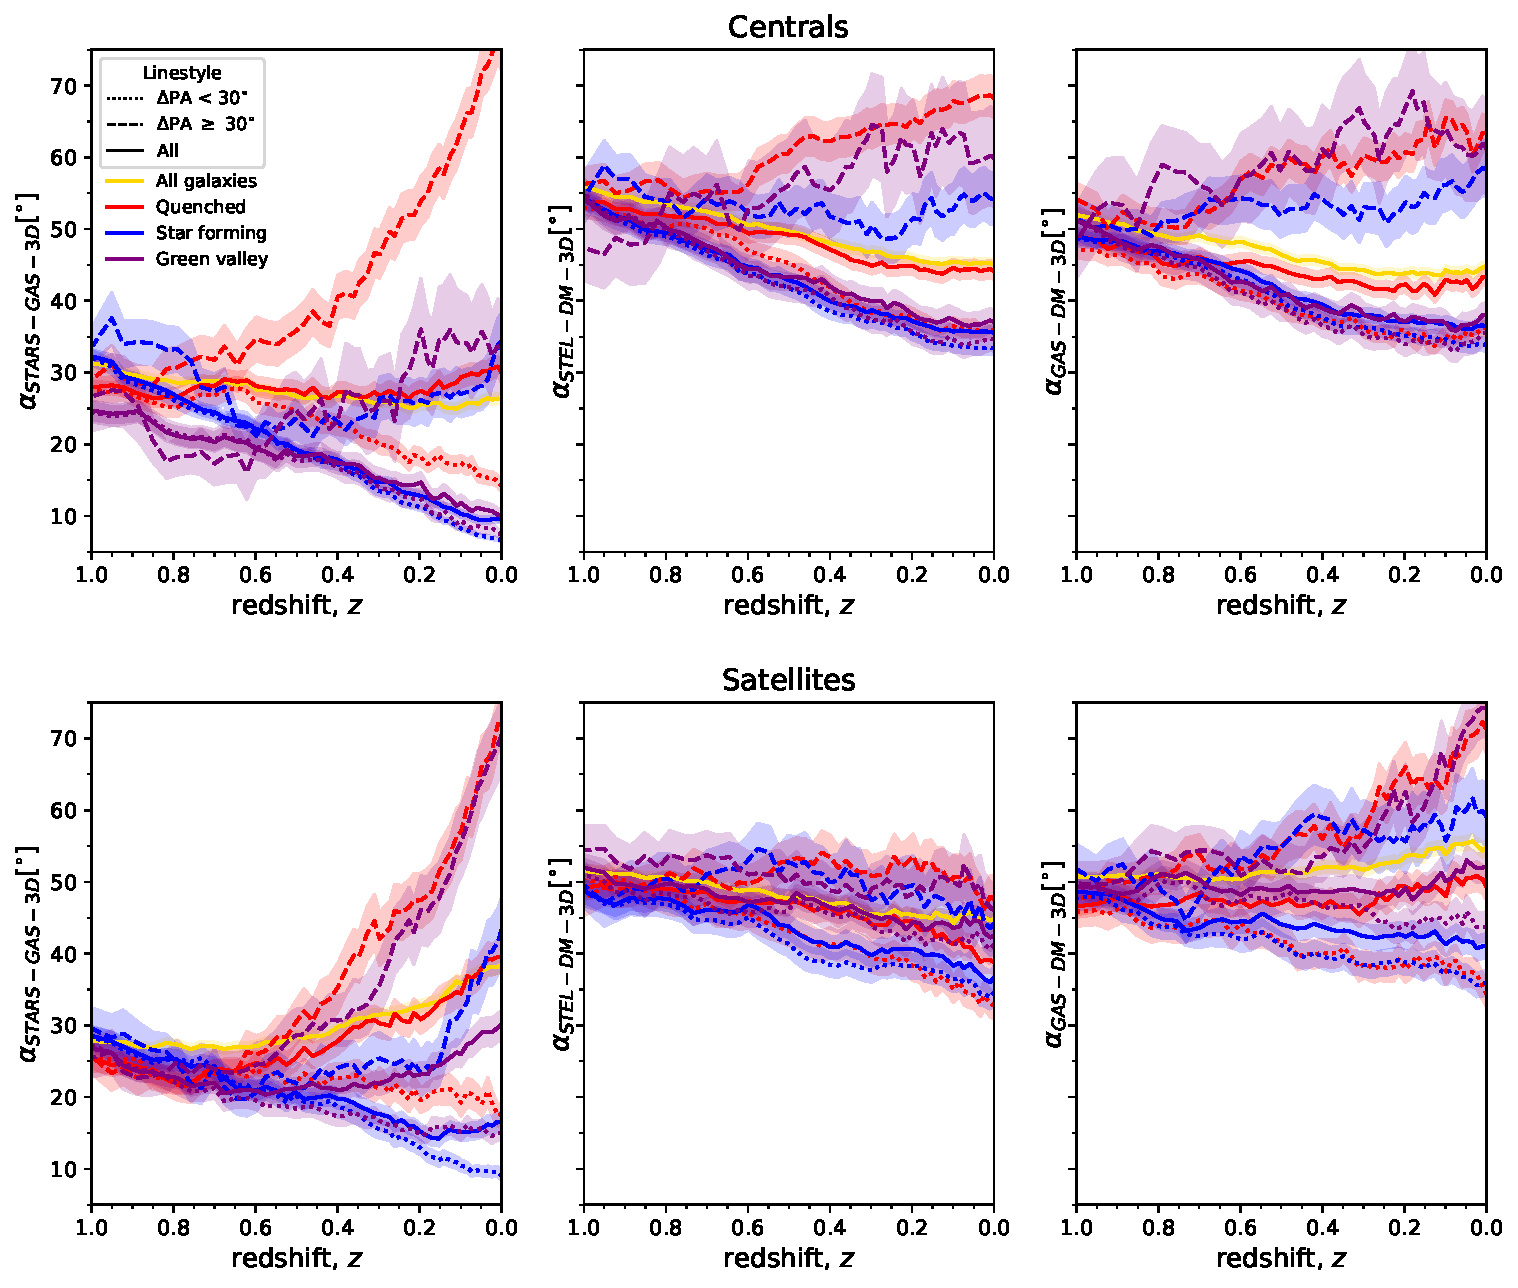
\includegraphics[width=\linewidth]{misalignment_TNG/3D_pa_evo_cen_sat.pdf}
    \caption{Evolution of the 3D offset (in degrees) between the principal spin axes of; stars and gas (left), stars and dark matter (middle) and gas and dark matter (right) from $z=1$. The evolution is taken as the median at each timestep for all galaxies of that category with errorbars showing the standard error. The top (bottom) row shows the evolution for central (satellite) galaxies. Each panel displays the evolution split into morphologies; quenched (red), green valley (purple) and star forming (blue) and also $\Delta$PA $< 30^{\circ}$ (dotted) and $\geq 30^{\circ}$ (dashed).}
    \label{fig:3D_alpha_evo}
\end{figure*}

\subsection{Summary of simulations} \label{sec:tng_summary}
In this work, we construct a mock MaNGA sample in IllustrisTNG100 to compare directly to observations and understand the build up of angular momentum in kinematically misaligned galaxies. Our conclusions are as follows:
\begin{enumerate}
    \item We find that a mock MaNGA like sample constructed from cosmological scale hydrodynamical simulation IllustrisTNG100 reproduces the observed trends of decoupling with morphology and stellar angular momentum at $z=0$.
    
    \item We find that decoupled galaxies reside in dark matter haloes with lower spin going back past $z=1$. Despite the decoupling between gas and stars being inherently transient in nature, it is also associated with a decoupling of both stars and gas with respect to dark matter. This demonstrates the inherent link of decoupling, not only to present day stellar angular momentum, but to lower spin haloes at $z=1$. 

\end{enumerate}

\section{Discussion} \label{sec:tng_discussion}
In this chapter we have demonstrated the relationship of kinematic misalignment with morphology, stellar angular momentum and dark matter halo spin. In the following we put our results in context and highlight the potential of using the decoupling of star-gas rotation to identify underlying properties of a galaxy. 

We note the close relationship of our findings of our samples with respect to the work of \citet{starkenburg+19}. They investigate the origin of star-gas decoupling (in this instance $ > 90^{\circ}$) using low mass galaxies (i.e. $2 \times \mathrm{10^{9} < M_{\ast} < 5 \times 10^{10}}$) in the original Illustris simulation. Despite extending the mass range and only considering the ensemble average for aligned and misaligned galaxies split at $\Delta$PA$ = 30^{\circ}$, we still find the same qualitative trends of lower angular momentum and lower gas mass fractions for misaligned galaxies (in comparison to aligned). 

While outside the scope of this work, we note that their estimation of relaxation timescales (i.e. until realignment of rotation axes) is of the order Gigayears. This appears to be roughly comparable to toy-model estimates \citep[see;][albeit for ETGs]{davis2016}. Here we also demonstrate the transient nature of star-gas decoupling (left panels, Figure \ref{fig:3D_alpha_evo}). Working back from $z=0$, we note that $\mathrm{\alpha_{STARS - GAS}}$ for the aligned and misaligned samples (at $z=0$) converges in the majority of cases before $z=1$. Since we are only considering the ensemble average for misalignment selected at $z=0$, we cannot comment on the timescales of misalignment here since the average may include several events that decouple the rotation.

In contrast, we see that the magnitude of specific angular momentum for stars, gas and DM for misaligned objects (at $z=0$) remains fundamentally lower going to at least $z=1$. This suggests that while star-gas misalignment at $z=0$ is a transient property, \textit{its likelihood is correlated with the angular momentum content of the halo at early times}. In part, the correlation must be driven by the lower angular momentum content of the stellar component. This inherently leads to longer relaxation timescales (i.e. longer star-gas decoupling) due to weaker stellar torques acting on the misaligned gas component and hence a higher likelihood of being misaligned at $z=0$.

We note the apparent relationship of misalignment with the different evolution of low and high spin haloes due to environment. In Horizon-AGN, \citet{khim2019} show that the misalignment fraction strongly increases in cluster environments. While not explicitly shown in this work, we find that misaligned satellites are typically closer to group centres, indicating the importance of gas stripping or interactions. In observations, \citet{li2019} find that at least 40\% of misalignment can be attributed to recent mergers or interactions. The environment of a given galaxy, modulating the probability of mergers/interactions and hence the spin of the halo/galaxy appears to be an important factor in dictating the misalignment fraction. However, current studies of the environmental dependence of misalignment in observations are inconclusive \citep[e.g. preference for misalignment in overdensity vs isolation; Chapter 5 vs][]{jin2016}.

We also note TNG100's ability to not only reproduce a reasonable distribution of $\Delta$PA with respect to the MaNGA sample (Figure \ref{fig:total_pa_dist}) once accounting for variances in mass between the $\Delta$PA defined samples in MaNGA and TNG100, but also reproducing the strong trends with morphology found in observations (Figure \ref{fig:group_morph_PA}). Whether the trigger of misalignment is internal or external, it appears to be clearly linked to a lowered gas mass (Figure \ref{fig:delPA_gasM}). In the next chapter, we use our simulated sample to investigate the temporal connection between black hole activity and misalignment in IllustrisTNG100. 